% !TEX root = task-25.tex
% EGE 2027, task 25. Source IDs and URLs are kept in comments.
% Editable task bank. Append new BankTask blocks at the end of the document.
\documentclass[12pt,a4paper]{article}
\usepackage{physics-textbook}
\usepackage{graphicx,needspace}
\usetikzlibrary{decorations.pathmorphing}
\newif\ifShowSolutions
\ifdefined\TutorEdition
  \ShowSolutionstrue
\else
  \ShowSolutionsfalse % Change to \ShowSolutionstrue to display solutions.
\fi
\newcounter{banktask}
\newsavebox{\BankTaskBox}
\newcommand{\BankTaskContent}[3]{%
  \noindent\textbf{\thebanktask.}\quad #2\par
  \ifShowSolutions
    \Needspace{50mm}% Keep the solution heading with its opening text or diagram.
    #3\par
    \ifdefined\TutorEdition
      \ifcsname TutorSource#1\endcsname
        \nopagebreak\smallskip{\small\csname TutorSource#1\endcsname\par}%
      \fi
    \fi
  \fi
}
\newcommand{\BankTask}[3]{%
  \refstepcounter{banktask}\par\medskip
  \sbox{\BankTaskBox}{\begin{minipage}{\linewidth}%
    \BankTaskContent{#1}{#2}{#3}\end{minipage}}%
  \ifdim\dimexpr\ht\BankTaskBox+\dp\BankTaskBox\relax>\dimexpr\textheight-20mm\relax
    \Needspace{35mm}\BankTaskContent{#1}{#2}{#3}%
  \else
    \Needspace{\dimexpr\ht\BankTaskBox+\dp\BankTaskBox\relax}%
    \noindent\usebox{\BankTaskBox}\par
  \fi
  \medskip
}
\begin{document}


% Source 43128: https://phys-ege.sdamgia.ru/problem?id=43128
\BankTask{43128}{
\begin{center}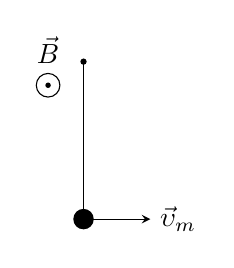
\begin{tikzpicture}[>=stealth]

\draw (0,2)--(0,0);\fill (0,2) circle(.04) (0,0) circle(.13);
\draw (-.45,1.7) circle(.15) node[above=.15cm]{$\vec B$};\fill (-.45,1.7) circle(.035);
\draw[->] (0,0)--(.85,0) node[right]{$\vec\upsilon_m$};
\end{tikzpicture}\end{center}
В однородном магнитном поле вращается по окружности в вертикальной плоскости положительно заряженный шарик массой m и зарядом q. Длина нити равна l. Минимальная скорость шарика в нижней точке, при которой шарик сможет совершить полный оборот, равна \ensuremath{\upsilon}. Найдите индукцию магнитного поля B.
}{
\smallskip\noindent\textbf{Решение}\par
\begin{center}\begin{tikzpicture}[>=stealth]

\draw (0,0) circle(1.4) (0,-1.4)--(0,1.4);\fill (0,-1.4) circle(.07) (0,0) circle(.05) (0,1.4) circle(.07);
\draw[->] (0,1.4)--(0,2.25) node[right]{$\vec F_{\!\text{л}}$};\draw[->] (0,1.4)--(0,.82) node[right]{$m\vec g$};
\draw[->] (0,.67)--(0,.29) node[right]{$\vec a$};\draw[->] (0,1.4)--(-.85,1.4) node[left]{$\vec\upsilon_2$};
\draw[->] (0,-1.4)--(.85,-1.4) node[right]{$\vec\upsilon_1$};\fill (-1.85,1.4) circle(.04) node[right]{$\vec B$};
\end{tikzpicture}\end{center}
При движении положительно заряженного тела магнитное поле действует на него с силой Лоренца, равной $F_{\,\text{л}}=Bq v \sin \alpha ,$ где $\sin \alpha =1,$ направление которой определяется правилом левой руки.
Рассмотрим движение заряженного шарика в магнитном и гравитационном поле. За нулевой уровень высоты примем нижнюю точку расположения шарика. В нижней точке он обладает кинетической энергией $E_{\,\text{к}1}= \frac{m v _1 ^2}{2} ,$  в верхней  — кинетической $E_{\,\text{к}2}= \frac{m v _2 ^2}{2}$ и потенциальной $E_{\,\text{п}2}=mgh=2mgl,$ где $v _2$ — скорость шарика в верхней точке. 
Так как сила Лоренца перпендикулярна вектору скорости, то работу не совершает. Тогда применим закон сохранения энергии:

\[\frac{m v _1 ^2}{2} = \frac{m v _2 ^2}{2} + 2mgl. ( 1 )\]

Так как шарику придали минимальную скорость, чтобы он совершил оборот в вертикальной плоскости, то в верхней точке сила натяжения нити равна $0$. На шарик в верхней точке действуют сила тяжести, сила Лоренца, направленная вверх. Под действием этих сил шарик имеет в верхней точке центростремительное ускорение $a= \frac{v _2 ^2}{R} = \frac{v _2 ^2}{l} .$
По второму закону Ньютона $m \vec{g} + \vec F_{\,\text{л}}=m \vec{a}.$ В проекции на вертикальную ось, направленную вниз получаем:

$mg - F_{\,\text{л}}=ma$
$Bq v _2=mg - \frac{m v _2 ^2}{l} . ( 2 )$

Объединяя формулы ($1$) и ($2$), находим индукцию магнитного поля:

\[B= \frac{m ( 5gl - v _1 ^2 )}{ql \sqrt{v _1 ^2 - 4gl}} .\]

Ответ: $B= \frac{m ( 5gl - v _1 ^2 )}{ql \sqrt{v _1 ^2 - 4gl}}$
}

% Source 41154: https://phys-ege.sdamgia.ru/problem?id=41154
\BankTask{41154}{
\begin{center}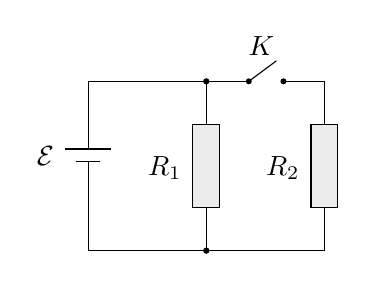
\begin{tikzpicture}[>=stealth]

\draw (0,0)--(3,0)--(3,.55) (3,1.6)--(3,2.15)--(2.48,2.15) (2.04,2.15)--(0,2.15)--(0,1.29) (0,1.13)--(0,0);
\draw (-.29,1.29)--(.29,1.29) (-.15,1.13)--(.15,1.13);
\node[left]at(-.31,1.2){$\mathcal E$};
\draw(1.5,0)--(1.5,.55) (1.5,1.6)--(1.5,2.15);
\draw(2.04,2.15)--(2.39,2.41);\node[above]at(2.2,2.35){$K$};
\fill(1.5,2.15)circle(.04) (1.5,0)circle(.04) (2.04,2.15)circle(.038) (2.48,2.15)circle(.038);
\draw[fill=gray!15] (1.33,.55)rectangle(1.67,1.6) (2.83,.55)rectangle(3.17,1.6);
\node[left]at(1.31,1.05){$R_1$};\node[left]at(2.81,1.05){$R_2$};
\end{tikzpicture}\end{center}
В электрической цепи, схема которой изображена на рисунке, ключ К сначала был разомкнут, а затем его замкнули. На сколько после этого изменилась тепловая мощность P, выделяющаяся в резисторе сопротивлением $R_{1}$  =  $10\,\text{Ом}$, если ЭДС батарейки равна $\mathcal E =12\,\text{В},$ её внутреннее сопротивление r  =  $2\,\text{Ом}$, а сопротивление резистора $R_{2}$  =  $15\,\text{Ом}$? Ответ дайте с учётом знака.
}{
\smallskip\noindent\textbf{Решение}\par
$1$.  До замыкания ключа К в левой части цепи по закону Ома для полной цепи течёт ток $I_1 = \frac{\mathcal E}{r + R_1} = 1\,\text{А},$ и в резисторе $R_{1}$ выделяется тепловая мощность $P_1 = I_1 ^2 R_1 = \frac{\mathcal E ^2 R_1}{( r + R_1 ) ^2} = 10\,\text{Вт}.$
$2$.  После замыкания ключа ток течёт уже через оба резистора $R_{1}$ и $R_{2}$. Согласно закону Ома для полной цепи, через батарейку течёт ток $I_2 = \frac{\mathcal E}{r + \frac{R_1R_2}{R_1 + R_2}} = 1{,}5\,\text{А}.$ При этом оба резистора $R_{1}$ и $R_{2}$ находятся под напряжением 

\[U_2 = \mathcal E - I_2r = \frac{\frac{ER_1R_2}{R_1 + R_2}}{r + \frac{R_1R_2}{R_1 + R_2}} = I_2 \frac{R_1R_2}{R_1 + R_2} .\]

$3$.  В резисторе $R_{1}$ при этом выделяется мощность 

\[P_2 = \frac{U_2 ^2}{R_1} = I_2 ^2 \frac{R_1R_2 ^2}{( R_1 + R_2 ) ^2} = 8{,}1\,\text{Вт}.\]

$4$.  Таким образом, изменение мощности после замыкания ключа равно: 

\[\Delta P = P_2 - P_1 = - 1{,}9\,\text{Вт}.\]

Ответ: $\Delta P = - 1{,}9\,\text{Вт}.$
}

% Source 16873: https://phys-ege.sdamgia.ru/problem?id=16873
\BankTask{16873}{
\begin{center}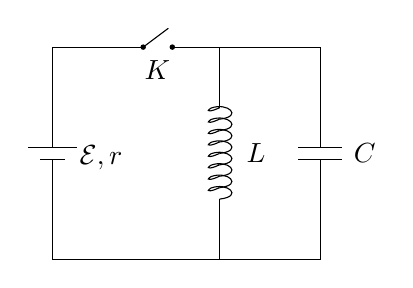
\begin{tikzpicture}[>=stealth]

\draw (0,0)--(3.4,0)--(3.4,1.27) (3.4,1.43)--(3.4,2.7)--(1.52,2.7) (1.15,2.7)--(0,2.7)--(0,1.43) (0,1.27)--(0,0)
(-.31,1.43)--(.31,1.43) (-.16,1.27)--(.16,1.27) (3.12,1.27)--(3.68,1.27) (3.12,1.43)--(3.68,1.43);
\draw(1.15,2.7)--(1.47,2.94);\fill (1.15,2.7)circle(.035) (1.52,2.7)circle(.035);
\node[below]at(1.33,2.65){$K$};\node[right]at(.22,1.30){$\mathcal E,r$};\node[right]at(3.7,1.35){$C$};
\draw (2.12,0)--(2.12,.77) (2.12,1.93)--(2.12,2.7);
\foreach \y in {.77,.915,1.06,1.205,1.35,1.495,1.64,1.785}{
 \begin{scope}[shift={(2.12,\y)}]\draw(0,0)..controls(.31,.035)and(.10,.22)..(-.11,.14)..controls(-.2,.08)and(-.08,.105)..(0,.145);\end{scope}}
\node[right]at(2.34,1.35){$L$};
\end{tikzpicture}\end{center}
В электрической цепи, показанной на рисунке, ключ К длительное время замкнут, $\mathcal E = 3\,\text{В},$ r = $2\,\text{Ом}$, L = $1$ мГн, С = $50$ мкФ. В момент t = $0$ ключ К размыкают. Каково напряжение U на конденсаторе в момент, когда в ходе возникших в контуре электромагнитных колебаний сила тока в контуре I = $1\,\text{А}$? Сопротивлением проводов и активным сопротивлением катушки индуктивности пренебречь.
}{
\smallskip\noindent\textbf{Решение}\par
Пока ключ замкнут через катушку течет постоянный ток $I_0,$ определяемый сопротивлением источника: $I_0 = \frac{\mathcal E}{r} .$ Поскольку активное сопротивление катушки, по условию, равно нулю, на катушке не падает напряжение, а значит, нулевое напряжение приложено к конденсатору. Таким образом, до размыкания ключа конденсатор разряжен. Начальная энергия электромагнитного поля в катушке $\frac{LI_0 ^2}{2} .$
После размыкания ключа начинаются электромагнитные колебания, и вся энергия, запасенная в катушке, будет перетекать из катушки в конденсатор и обратно. Энергия конденсатора равна $\frac{CU ^2}{2} .$ Через некоторое время энергия катушки уменьшится, а энергия конденсатора увеличится, причем сумма этих энергий будет равна начальной энергии катушки:

\[\frac{LI_0 ^2}{2} = \frac{LI ^2}{2} + \frac{CU ^2}{2} .\]

Откуда:

\[U = \sqrt{\frac{L ( I_0 ^2 - I ^2 )}{C}} = \sqrt{\frac{10^{-3} \,\text{Гн} \cdot \bigl( ( \frac{3\,\text{В}}{2\,\text{Ом}} ) ^2 - ( 1\,\text{А} ) ^2 \bigr)}{50 \cdot 10 ^{ - 6 } \,\text{Ф}}} = 5\,\text{В}.\]

Ответ: $5\,\text{В}$.
}

% Source 43126: https://phys-ege.sdamgia.ru/problem?id=43126
\BankTask{43126}{
К решетке вплотную поставили линзу, которая собирает лучи в одной точке на экране. Линза расположена между решеткой и экраном. Расстояние от линзы до экрана $2\,\text{м}$. Ширина спектра второго порядка $8\,\text{см}$. Длина волны красного света $8$ · $10^{-7}$ и фиолетового света $4$ · $10^{-7}$ м. Найдите, сколько штрихов приходится на $1\,\text{см}$ решетки. $\sin \varphi \approx \tan \varphi \approx \varphi.$
}{
\smallskip\noindent\textbf{Решение}\par
Условие дифракционного максимума $d \sin \varphi =k\lambda,$ где для малых углов $\sin \varphi \approx \tan \varphi = \frac{b}{L} .$
Тогда для максимума фиолетового и красного света получаем

$\frac{db_1}{L} =k\lambda_1$
$\frac{db_2}{L} =k\lambda_2.$

Откуда находим период решетки:

\[d= \frac{Lk ( \lambda_1 - \lambda_2 )}{\Delta b} = \frac{2 \cdot 2 \cdot ( 8 \cdot 10 ^{ - 7 } - 4 \cdot 10 ^{ - 7 } )}{8 \cdot 10 ^{ - 2 }} =2 \cdot 10 ^{ - 5 } \,\text{м}=2 \cdot 10 ^{ - 3 } \,\text{см}.\]

Тогда на $1\,\text{см}$ приходится количество штрихов:

\[N= \frac{1\,\text{см}}{d} = \frac{1}{2 \cdot 10 ^{ - 3 }} =500.\]

Ответ: $500$.
}

% Source 39266: https://phys-ege.sdamgia.ru/problem?id=39266
\BankTask{39266}{
\begin{center}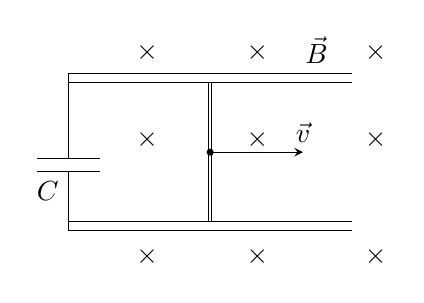
\begin{tikzpicture}[>=stealth]

\draw (0,.92)--(0,2)--(3.6,2) (0,.76)--(0,0)--(3.6,0) (-.4,.76)--(.4,.76) (-.4,.92)--(.4,.92);
\draw (0,1.88)--(3.6,1.88) (0,.12)--(3.6,.12);\draw[double] (1.8,.12)--(1.8,1.88);
\node[below left]at(0,.75){$C$};\draw[->] (1.8,1)--(2.98,1)node[above]{$\vec v$};\fill (1.8,1)circle(.045);
\foreach \x in {1,2.4,3.9}{\foreach \y in {-.32,1.16,2.26}{\node at(\x,\y){$\times$};}}
\node[above]at(3.15,2){$\vec B$};
\end{tikzpicture}\end{center}
По двум горизонтально расположенным параллельным проводящим рельсам с пренебрежимо малым сопротивлением, замкнутым на конденсатор электроёмкостью С  =  $100$ мкФ, поступательно и равномерно скользит проводящий стержень. Расстояние между рельсами l  =  $1\,\text{м}$. Рельсы со стержнем находятся в вертикальном однородном магнитном поле с индукцией B  =  $1$ Тл (см. рис.). Через достаточно большой промежуток времени от начала движения энергия электрического поля конденсатора W  =  $50$ мкДж. Какова скорость движения стержня? Рельсы закреплены на диэлектрической подложке.
}{
\smallskip\noindent\textbf{Решение}\par
$1$.  Модуль ЭДС индукции, возникающей в контуре при движении стержня: $|\mathcal E|=B v l,$где B  — модуль вектора магнитной индукции, \ensuremath{\upsilon}  — скорость движения стержня, l  — длина стержня. 
$2$.  Так как напряжение на конденсаторе $U_{c}$ равно модулю ЭДС индукции, то энергия электрического поля конденсатора определяется по формуле: 

\[W= \frac{C U_C ^2}{2} = \frac{C B ^2 v ^2 l ^2}{2} .\]

В итоге скорость стержня равна: 

\[v = \sqrt{\frac{2 W}{C B ^2 l ^2}} = \sqrt{\frac{2 \cdot 50 \cdot 10^{-6}}{100 \cdot 10 ^{ - 6 } \cdot 1 ^2 \cdot 1 ^2}} =1 \,\text{м} / \,\text{с}.\]

Ответ: $1\,\text{м/с}$.
}

% Source 6668: https://phys-ege.sdamgia.ru/problem?id=6668
\BankTask{6668}{
На горизонтальной плоскости в вершинах правильного пятиугольника закреплены $5$ одинаковых положительных зарядов Q  =  $1$ мкКл, расположенные на расстоянии R  =  $2\,\text{м}$ от центра этого пятиугольника. На вертикальной прямой, проведенной из этого центра, на высоте $0{,}75$R над плоскостью находится положительный заряд q  =  $4$ мкКл. Найдите модуль и направление силы F, действующей на него со стороны остальных зарядов.
}{
\smallskip\noindent\textbf{Решение}\par
По закону Кулона сила f взаимодействия зарядов Q и q, находящихся на расстоянии r друг от друга, равна $f= \frac{1}{4 \pi \varepsilon_0} \cdot \frac{qQ}{r ^2} ,$ или в векторной форме: $\vec{f}= \frac{1}{4 \pi \varepsilon_0} \cdot \frac{qQ}{r ^3} \vec{r}.$
В нашем случае $r= \sqrt{R ^2 + 0{,}75 ^2 R ^2} =1{,}25R,f= \frac{1}{4 \pi \varepsilon_0} \cdot \frac{qQ}{1{,}5625R ^2} .$ Вектор $\vec{f}$ образует с вертикалью угол $\alpha$ такой, что $\cos \alpha = \frac{0{,}75R}{1{,}25R} =0{,}6.$
Проекции всех пяти векторов $\vec{f}$ на вертикальную ось одинаковы и равны $f_\parallel= \frac{1}{4 \pi \varepsilon_0} \cdot \frac{qQ}{r ^2} \cos \alpha ,$ а их проекции на направления, перпендикулярные оси, равны $f_\perp= \frac{1}{4 \pi \varepsilon_0} \cdot \frac{qQ}{r ^2} \sin \alpha .$
В соответствии с принципом суперпозиции сил сумма пяти одинаковых векторов $\vec{f}_\perp,$ образующих правильный пятиугольник, равна нулю, а сумма пяти одинаковых векторов $\vec{f}_\parallel,$ направленных вдоль оси, дает действующую на заряд q суммарную силу, равную по модулю:

\[F= \frac{1}{4 \pi \varepsilon_0} \cdot \frac{5 \cdot 0{,}6 \cdot qQ}{1{,}5625R ^2} = \frac{1{,}92}{4 \pi \varepsilon_0} \cdot \frac{qQ}{R ^2} =17{,}28\,\text{мН}\]

и направленную вдоль оси пятиугольника «от него».

Ответ: Сила направлена вдоль оси пятиугольника «от него» и по модулю равна $F= \frac{1{,}92}{4 \pi \varepsilon_0} \cdot \frac{qQ}{R ^2} =17{,}28\,\text{мН}.$
}

% Source 8025: https://phys-ege.sdamgia.ru/problem?id=8025
\BankTask{8025}{
\begin{center}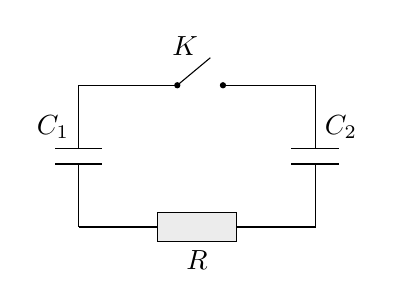
\begin{tikzpicture}[>=stealth]

\draw(0,0)--(1,0) (2,0)--(3,0)--(3,.8) (3,1)--(3,1.8)--(1.83,1.8) (1.25,1.8)--(0,1.8)--(0,1) (0,.8)--(0,0);
\draw(-.3,.8)--(.3,.8) (-.3,1)--(.3,1) (2.7,.8)--(3.3,.8) (2.7,1)--(3.3,1);
\draw[fill=gray!15](1,-.18)rectangle(2,.18);\draw(1.25,1.8)--(1.67,2.15);
\fill (1.25,1.8)circle(.04) (1.83,1.8)circle(.04);\node[above]at(1.35,2.05){$K$};\node[above left]at(0,1){$C_1$};\node[above right]at(3,1){$C_2$};\node[below]at(1.5,-.18){$R$};
\end{tikzpicture}\end{center}
Конденсатор $C_{1}$  =  $1$ мкФ заряжен до напряжения U  =  $300\,\text{В}$ и включен в последовательную цепь из резистора R  =  $300\,\text{Ом}$, незаряженного конденсатора $C_{2}$  =  $2$ мкФ и разомкнутого ключа К (см. рис.). Какое количество теплоты выделится в цепи после замыкания ключа, пока ток в цепи не прекратится?
}{
\smallskip\noindent\textbf{Решение}\par
После соединения конденсаторов напряжение U на них будет одинаковым. По закону сохранения заряда $q_1 + q_2=q_1' + q_2',$ где заряды до соединения на первом конденсаторе равен $q_1=C_1U_1,$ на втором конденсаторе $q_2=0,$ а заряды после соединения $q_1'=C_1U$ и $q_2'=C_2U.$ Откуда получаем:

\[C_1U_1=U ( C_1 + C_2 ) .\]

Энергии конденсаторов до и после соединения равнялись $W_1= \frac{C_1U_1 ^2}{2}$ и $W_2= \frac{( C_1 + \,\text{С}_2 ) U ^2}{2} .$ Выделившаяся на резисторе теплота равна $Q=W_1 - W_2.$
По закону сохранения энергии выделившееся в цепи количество теплоты равно разности значений энергии конденсаторов в начальном и конечном состояниях: 

\[Q= \frac{C_1U ^2}{2} - \frac{( C_1U ) ^2}{2 ( C_1 + C_2 )} .\]

Откуда получим:

\[Q= \frac{C_1C_2U ^2}{2 ( C_1 + C_2 )} = \frac{10 ^{ - 6 } \cdot 2 \cdot 10 ^{ - 6 } \cdot 300 ^2}{2 ( 10 ^{ - 6 } + 2 \cdot 10 ^{ - 6 } )} =0{,}03\,\text{Дж}.\]

Ответ: Q  =  $30\,\text{мДж}$.
}

% Source 9333: https://phys-ege.sdamgia.ru/problem?id=9333
\BankTask{9333}{
Плоская монохроматическая световая волна с частотой $8{,}0$ · $10^{14}$ Гц падает по нормали на дифракционную решетку. Параллельно решетке позади нее размещена собирающая линза с фокусным расстоянием $21\,\text{см}$. Дифракционная картина наблюдается на экране в задней фокальной плоскости линзы. Расстояние между ее главными максимумами $1$-го и $2$-го порядков равно $18\,\text{мм}$. Найдите период решетки. Ответ выразите в микрометрах (мкм), округлив до десятых. Считать для малых углов ($\varphi \ll 1$ в радианах) $\tan \varphi \approx \sin \varphi \approx \varphi.$
}{
\smallskip\noindent\textbf{Решение}\par
Запишем условия максимума для $1$-го и $2$-го порядков:

\[\begin{cases}d\sin\varphi_1=\lambda,\\d\sin\varphi_2=2\lambda.\end{cases}\quad\Longleftrightarrow\quad\begin{cases}\tan\varphi_1\approx\sin\varphi_1=\frac{\lambda}{d}=\frac{c}{\nu d},\\\tan\varphi_2\approx\sin\varphi_2=\frac{2\lambda}{d}=\frac{2c}{\nu d}.\end{cases}\]

На экране максимумы смещены на расстояния $x_1=f \tan \varphi_1$ и $x_2=f \tan \varphi_2$ от центрального максимума, где f  — фокусное расстояние линзы. По условию $x_2 - x_1=\Delta x = 18\,\text{мм}.$ Из чего получаем

\[\frac{2fc}{\nu d} - \frac{fc}{\nu d} =\Delta x \Longleftrightarrow d= \frac{fc}{\nu \Delta x} = \frac{0{,}21 \cdot 3 \cdot 10 ^{8}}{8{,}0 \cdot 10 ^{ 14 } \cdot 18 \cdot 10 ^{ - 3 }} \approx 4{,}4 \cdot 10 ^{ - 6 } \,\text{м} = 4{,}4\,\text{мкм}.\]

Ответ: $4{,}4$
}

% Source 3024: https://phys-ege.sdamgia.ru/problem?id=3024
\BankTask{3024}{
Горизонтальный проводящий стержень прямоугольного сечения поступательно движется с ускорением вверх по гладкой наклонной плоскости в вертикальном однородном магнитном поле (см. рис.).
\begin{center}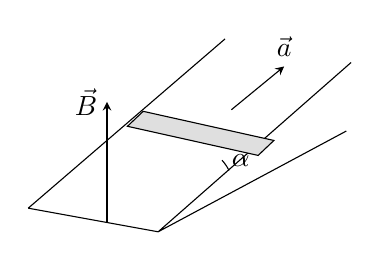
\begin{tikzpicture}[>=stealth]

\draw (0,.3)--(1.65,0)--(4.1,2.15) (0,.3)--(2.5,2.45) (1.65,0)--(4.04,1.28);
\draw (2.55,.78) arc(27:42:.6) node[right]{$\alpha$};
\draw[fill=gray!25] (1.26,1.34)--(2.92,.97)--(3.12,1.16)--(1.46,1.53)--cycle;
\draw[->] (2.58,1.55)--(3.25,2.1) node[above]{$\vec a$};\draw[->] (1,.13)--(1,1.65) node[left]{$\vec B$};
\end{tikzpicture}\end{center}

По стержню протекает ток I. Угол наклона плоскости $\alpha = 30 ^\circ.$ Отношение массы стержня к его длине $\frac{m}{L} =0{,}1\,\text{кг/м}.$ Модуль индукции магнитного поля $B = 0{,}2\,\text{Тл}.$ Ускорение стержня $a = 1{,}9\,\text{м/с} ^2 .$ Чему равна сила тока в стержне?
}{
\smallskip\noindent\textbf{Решение}\par
\begin{center}\begin{tikzpicture}[>=stealth]

\draw (0,0)--(3.2,0);\draw[->] (0,0)--(3.2,1.85) node[right]{$x$};\draw (.65,0)arc(0:30:.65)node[midway,right]{$\alpha$};
\draw[fill=gray!20,rotate=30] (1.1,0)rectangle(2,.43);
\coordinate (M) at (1.34,.79);\draw[->] (M)--(2.68,.79)node[right]{$\vec F_{\!\text{А}}$};
\draw[->] (M)--(.71,1.88) node[above]{$\vec N$};\draw[->] (M)--(1.34,-.55) node[below]{$m\vec g$};
\end{tikzpicture}\end{center}
$1$.  На рисунке показаны силы, действующие на стержень с током:
—  сила тяжести $m\vec{g},$ направленная вертикально вниз; 
—  сила реакции опоры $\vec{N},$ направленная перпендикулярно к наклонной плоскости;
—  сила Ампера $\vec F_{\,\text{А}},$ направленная горизонтально вправо, что вытекает из условия задачи.
$2$.  Модуль силы Ампера $F_{\,\text{А}}=IBL \sin \beta ,$ где  угол между направлением тока и вектором магнитной индукции $\sin \beta =1.$
$3$.  Систему отсчета, связанную с наклонной плоскостью, считаем инерциальной. Для решения задачи достаточно записать второй закон Ньютона $\vec{N} + \vec F_A + m \vec{g}=m \vec{a} .$ 
В проекциях на ось х (см. рис.):

\[ma= - mg \sin \alpha + IBL \cos \alpha .\]

Отсюда находим $I= \frac{m ( a + g \sin \alpha )}{LB \cos \alpha} = \frac{0{,}1 \cdot ( 1{,}9 + 10 \cdot \sin 30 ^\circ )}{0{,}2 \cdot \cos 30 ^\circ} \approx 4\,\text{А}.$

Ответ: $I\approx 4\,\text{А}.$
}

% Source 5737: https://phys-ege.sdamgia.ru/problem?id=5737
\BankTask{5737}{
Проволочная катушка сопротивлением $10\,\text{Ом}$ расположена в постоянном однородном магнитном поле так, что линии его индукции направлены вдоль оси катушки. Если соединить концы проволоки друг с другом и выключить магнитное поле, то через катушку протечет заряд $0{,}2\,\text{Кл}$. Найдите амплитуду ЭДС индукции, которая возникнет в катушке, если вновь включить прежнее магнитное поле и начать вращать в нем катушку с угловой скоростью $3\,\text{рад/с}$. Ось вращения перпендикулярна оси катушки. Ответ приведите в вольтах.
}{
\smallskip\noindent\textbf{Решение}\par
По закону Фарадея изменение магнитного потока, пронизывающего замкнутый проводящий контур, во времени, приводит к возникновению ЭДС индукции $\mathcal E_i = - \frac{\Delta \Phi}{\Delta t} .$
C другой стороны, по закону Ома ЭДС индукции выражается через силу тока в контуре и сопротивление контура
$I= \frac{\mathcal E _i}{R} .$ По определению силы тока $I= \frac{\Delta q}{\Delta t} .$
Поэтому $- \Delta \Phi = \Phi - 0 = \Delta qR.$ Здесь $\Phi$  — магнитный поток, пронизывавший катушку до выключения поля. 
При вращении катушки поток будет изменяться по закону $\Phi_1=\Phi \cos \omega t,$ следовательно: 

\[\mathcal E_i = - \Phi'_t = \Phi \omega \sin \omega t=\Delta qR\omega \sin \omega t.\]

Следоватеьно, амплитуда ЭДС индукции равна $\mathcal E_{\max}=\Delta qR\omega =0{,}2\,\text{Кл} \cdot 10\,\text{Ом} \cdot 3\,\text{рад/с}=6\,\text{В}.$

Ответ: $6\,\text{В}$.
}

% Source 43028: https://phys-ege.sdamgia.ru/problem?id=43028
\BankTask{43028}{
В вакууме в однородное горизонтальное электрическое поле с напряженностью E  =  $1000$ кВ/м помещают неподвижную капельку массой m  =  $0{,}4\,\text{г}$ и зарядом q  =  $3\,\text{нКл}$. Определите скорость капельки через t  =  $0{,}2\,\text{с}$. Сделайте рисунок, на котором укажите силы, действующие на капельку.
}{
\smallskip\noindent\textbf{Решение}\par
\begin{center}\begin{tikzpicture}[>=stealth]

\draw[->](-.65,1.05)--(2.55,1.05)node[midway,above]{$\vec E$};
\fill (0,.38) circle(.055);\draw[->](0,.38)--(1.25,.38) node[right]{$\vec F_{\!\text{э}}$};\draw[->](0,.38)--(0,-.65)node[below]{$m\vec g$};
\end{tikzpicture}\end{center}
На капельку действуют сила тяжести $m \vec{g}$ и сила действия электрического поля, направленная по линиям напряженности и равная $F_{\,\text{э}}=Eq.$
Равнодействующая этих сил постоянна и по второму закону Ньютона равна 

\[m \vec{g} + \vec F_{\,\text{э}}=m \vec{a} .\]

По горизонтальной оси: проекция ускорения капельки

\[a_x= \frac{Eq}{m} ,\]

тогда проекция скорости на горизонтальную ось при равноускоренном движении без начальной скорости

\[v _x= a_xt= \frac{Eqt}{m} .\]

По вертикали под действием силы тяжести $a_y=g,$ поэтому вертикальная проекция скорости капельки равна 

\[v _y=gt.\]

Тогда скорость капли через промежуток времени t равна

\[v = \sqrt{v _x ^2 + v _y ^2} =t \sqrt{( \frac{Eq}{m} ) ^2 + g ^2} =0{,}2 \cdot \sqrt{( \frac{3 \cdot 10^{-9} \cdot 10^{6}}{4 \cdot 10 ^{ - 4 }} ) ^2 + 100} =2{,}5 \,\text{м/с} .\]

Ответ: $2{,}5\,\text{м/с}$.
}

% Source 11955: https://phys-ege.sdamgia.ru/problem?id=11955
\BankTask{11955}{
\begin{center}\begin{tikzpicture}[>=stealth]

\draw[step=.5,gray!55] (0,-1.5)grid(3,2.5);
\draw[->] (0,-1.5)--(0,2.58) node[above left]{$B_{\text{п}},\,\text{Тл}$};\draw[->] (0,0)--(3.08,0) node[right]{$t,\,\text{с}$};
\draw[thick](0,1.5)--(1,-1)--(2.5,.5);\node[below left] at(0,0){$0$};
\foreach \y/\t in {-.5/{-0{,}2},-1/{-0{,}4},.5/{0{,}2},1/{0{,}4},1.5/{0{,}6}}{\node[left]at(0,\y){$\t$};}
\node[below]at(1,0){$4$};\node[below]at(2,0){$8$};
\end{tikzpicture}\end{center}
Квадратная проволочная рамка со стороной l  =  $10\,\text{см}$ находится в однородном магнитном поле с индукцией $\vec{B}.$ На рисунке изображена зависимость проекции вектора $\vec{B}$ на перпендикуляр к плоскости рамки от времени. Какое количество теплоты выделится в рамке за время t  =  $10\,\text{с}$, если сопротивление рамки R  =  $0{,}2\,\text{Ом}$?
}{
\smallskip\noindent\textbf{Решение}\par
При изменении магнитного поля изменяется поток вектора магнитной индукции $\,\text{Ф} ( t ) = B ( t ) S$ через рамку площадью $S = l ^2 ,$ что создает в ней ЭДС индукции $\mathcal E.$ В соответствии с законом индукции Фарадея:

\[\mathcal E = - \frac{\Delta \,\text{Ф}}{\Delta t} .\]

Эта ЭДС вызывает в рамке ток, сила которого определяется законом Ома для замкнутой цепи: 

\[I= \frac{\mathcal E}{R} .\]

Согласно закону Джоуля  — Ленца за время $\Delta$t в рамке выделится количество теплоты:

\[Q = I ^2 R\Delta t .\]

Таким образом, количество теплоты, выделяющееся в рамке, равно:

\[Q= \frac{l ^{4}}{R} \cdot \frac{( \Delta B_n ) ^2}{\Delta t} .\]

На первом участке графика $\Delta t = t_1 = 4\,\text{с}$ и $\Delta B = B_1 - B_0 = - 1\,\text{Тл},$ на втором участке $\Delta t_2 = t_2 - t_1 = 6\,\text{с}$ и $\Delta B = B_2 - B_1 = 0{,}6\,\text{Тл},$ поэтому суммарное количество выделившейся теплоты:

\[Q = Q_1 + Q_2 = \frac{l ^{4}}{R} \left[ \frac{( \Delta B_1 ) ^2}{\Delta t_1} + \frac{( \Delta B_2 ) ^2}{\Delta t_2} \right] .\]

Подставляя сюда значения физических величин, получим:

\[Q = \frac{( 0{,}1\,\text{м} ) ^{4}}{0{,}2\,\text{Ом}} \cdot \left[ \frac{1\,\text{Тл} ^2}{4\,\text{с}} + \frac{0{,}36\,\text{Тл} ^2}{6\,\text{с}} \right] = 0{,}155 \cdot 10 ^{ - 3 } \,\text{Дж}.\]

Ответ: $0{,}155\,\text{мДж}$.
}

% Source 43830: https://phys-ege.sdamgia.ru/problem?id=43830
\BankTask{43830}{
\begin{center}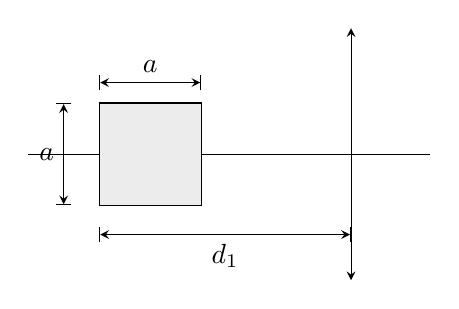
\begin{tikzpicture}[>=stealth]

\draw (-4.1,0)--(1,0);\draw[<->](0,-1.6)--(0,1.6);
\draw[fill=gray!15](-3.2,-.65)rectangle(-1.9,.65);
\draw[|<->|](-3.2,.91)--(-1.9,.91)node[midway,above]{$a$};
\draw[|<->|](-3.65,-.65)--(-3.65,.65)node[midway,left]{$a$};
\draw[|<->|](-3.2,-1.02)--(0,-1.02)node[midway,below]{$d_1$};
\end{tikzpicture}\end{center}
Квадрат со стороной a  =  $20\,\text{см}$ расположен в плоскости главной оптической оси тонкой собирающей линзы с оптической силой D  =  $2\,\text{дптр}$ так, что две его стороны параллельны плоскости линзы (см. рис.). Расстояние от дальней стороны квадрата до плоскости линзы $d_{1}$  =  $90\,\text{см}$. Определите площадь изображения квадрата в линзе. Сделайте рисунок, на котором постройте изображение квадрата в линзе, указав ход всех необходимых для построения лучей.
}{
\smallskip\noindent\textbf{Решение}\par
Обозначим вершины квадрата ABCD, тогда AB  =  AD  =  a.  
Для построения изображения квадрата проведём побочные оптические оси AO и BO, а также луч AB, параллельный главной оптической оси, который, преломившись, пройдёт через фокус линзы. В силу симметрии предмета относительно главной оптической оси его изображение также будет симметричным. В результате построений получим изображение квадрата ABCD в виде равнобедренной трапеции $A_{1}$$B_{1}$$C_{1}$$D_{1}$ (см. рис.).
\begin{center}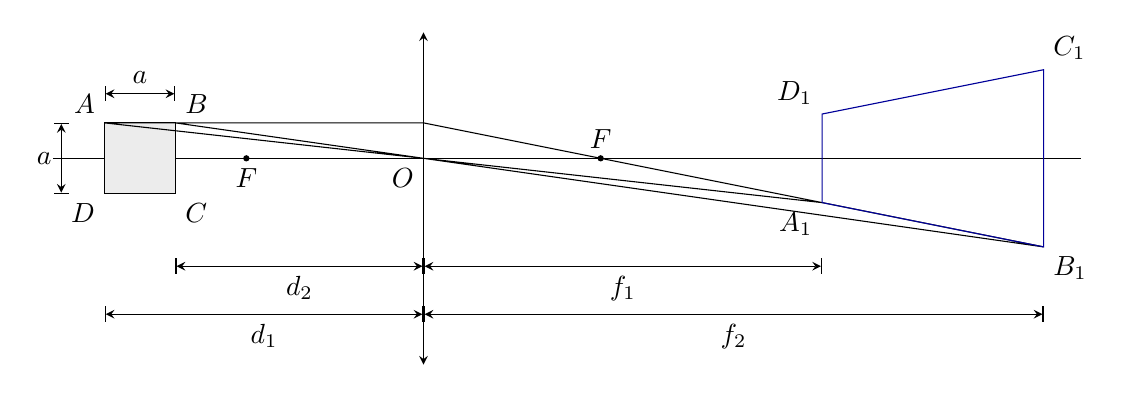
\begin{tikzpicture}[>=stealth]

\draw (-4.7,0)--(8.35,0);\draw[<->](0,-2.62)--(0,1.6);\node[below left] at(0,0){$O$};
\draw[fill=gray!15](-4.05,-.45)rectangle(-3.15,.45);
\node[above left]at(-4.05,.45){$A$};\node[above right]at(-3.15,.45){$B$};
\node[below right]at(-3.15,-.45){$C$};\node[below left]at(-4.05,-.45){$D$};
\fill (-2.25,0)circle(.04) node[below]{$F$} (2.25,0)circle(.04)node[above]{$F$};
\draw (-4.05,.45)--(0,.45)--(7.875,-1.125) (-4.05,.45)--(5.0625,-.5625) (-3.15,.45)--(7.875,-1.125);
\draw[blue!60!black] (5.0625,-.5625)--(7.875,-1.125)--(7.875,1.125)--(5.0625,.5625)--cycle;
\node[below left]at(5.0625,-.5625){$A_1$};\node[below right]at(7.875,-1.125){$B_1$};
\node[above right]at(7.875,1.125){$C_1$};\node[above left]at(5.0625,.5625){$D_1$};
\draw[|<->|](-4.05,.82)--(-3.15,.82)node[midway,above]{$a$};
\draw[|<->|](-4.6,-.45)--(-4.6,.45)node[midway,left]{$a$};
\draw[|<->|](-3.15,-1.37)--(0,-1.37)node[midway,below]{$d_2$};
\draw[|<->|](0,-1.37)--(5.0625,-1.37)node[midway,below]{$f_1$};
\draw[|<->|](-4.05,-1.98)--(0,-1.98)node[midway,below]{$d_1$};
\draw[|<->|](0,-1.98)--(7.875,-1.98)node[midway,below]{$f_2$};
\end{tikzpicture}\end{center}

Согласно формуле оптической силы линзы $F = \frac{1}{D} = \frac{1}{2} = 0{,}5 \,\text{м} = 50 \,\text{см}.$ Расстояние от линзы до квадрата равно $d_2 = d_1 - a = 90 - 20 = 70 \,\text{см}.$ По формуле тонкой линзы определим расстояния от линзы до оснований трапеции:

$\frac{1}{F} = \frac{1}{d_1} + \frac{1}{f_1} ,$
$\frac{1}{F} = \frac{1}{d_2} + \frac{1}{f_2} .$

 В итоге

$f_1 = \frac{Fd_1}{d_1 - F} = \frac{50 \cdot 90}{90 - 50} = 112{,}5 \,\text{см},$
$f_2 = \frac{Fd_2}{d_2 - F} = \frac{50 \cdot 70}{70 - 50} = 175 \,\text{см}.$

 Высота трапеции $h = f_2 - f_1 = 62{,}5 \,\text{см}.$
Используя формулу увеличения линзы для двух сторон квадрата, получим

$\frac{AD}{d_1} = \frac{A_1D_1}{f_1} ,$
$\frac{BC}{d_2} = \frac{B_1C_1}{f_2} .$

 Следовательно,

$A_1D_1 = \frac{f_1 \cdot AD}{d_1} = \frac{112{,}5 \cdot 20}{90} = 25 \,\text{см},$
$B_1C_1 = \frac{f_2 \cdot BC}{d_2} = \frac{175 \cdot 20}{70} = 50 \,\text{см}.$

Площадь изображения (трапеции) определяется формулой

\[S = \frac{A_1D_1 + B_1C_1}{2} \cdot h = \frac{25 + 50}{2} \cdot 62{,}5 \approx 2344 \,\text{см} ^2 .\]

Ответ: $S \approx 2344 \,\text{см} ^2 .$
}

% Source 4756: https://phys-ege.sdamgia.ru/problem?id=4756
\BankTask{4756}{
\begin{center}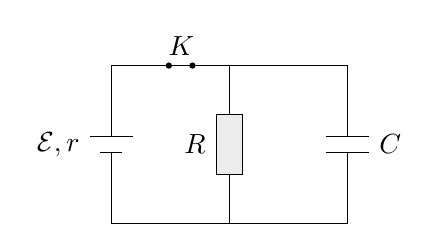
\begin{tikzpicture}[>=stealth]

\draw(0,0)--(3,0)--(3,.9) (3,1.1)--(3,2)--(1.03,2) (.73,2)--(0,2)--(0,1.1) (0,.9)--(0,0);
\draw(.73,2)--(1.03,2);\fill(.73,2)circle(.04) (1.03,2)circle(.04);\node[above]at(.89,2){$K$};
\draw(-.27,1.1)--(.27,1.1) (-.14,.9)--(.14,.9) (2.73,1.1)--(3.27,1.1) (2.73,.9)--(3.27,.9);
\draw(1.5,0)--(1.5,.62) (1.5,1.38)--(1.5,2);\draw[fill=gray!15](1.33,.62)rectangle(1.67,1.38);
\node[left]at(-.28,1){$\mathcal E,r$};\node[left]at(1.32,1){$R$};\node[right]at(3.28,1){$C$};
\end{tikzpicture}\end{center}
В электрической схеме, показанной на рисунке, ключ К замкнут. ЭДС батарейки $\mathcal E = 12\,\text{В},$ емкость конденсатора $C = 0{,}2\,\text{мкФ}.$ Отношение внутреннего сопротивления батарейки к сопротивлению резистора $k= \frac{r}{R} =0{,}2.$ Найдите количество теплоты, которое выделится на резисторе после размыкания ключа К в результате разряда конденсатора.
}{
\smallskip\noindent\textbf{Решение}\par
Когда ключ замкнут, конденсатор заряжен, а через резистор течет ток, который можно найти, применив закон Ома для полной цепи:

\[I= \frac{\mathcal E}{R + r} .\]

Поскольку резистор и конденсатор подключены параллельно, напряжения на них совпадают и равны:

\[U = IR = \frac{R \mathcal E}{R + r} .\]

После размыкания ключа, конденсатор разряжается через сопротивление, и вся накопленная в нем энергия электрического поля переходит в тепло. Таким образом, искомое количество теплоты равно:

\[Q= \frac{CU ^2}{2} = \frac{C}{2} ( \frac{\mathcal E}{1 + r/R} ) ^2 = \frac{0{,}2 \cdot 10 ^{ - 6 } \,\text{Ф}}{2} \cdot ( \frac{12\,\text{В}}{1 + 0{,}2} ) ^2 = 10 ^{ - 5 } \,\text{Дж}.\]

Ответ: $10 ^{ - 5 } \,\text{Дж}.$
}

% Source 50816: https://phys-ege.sdamgia.ru/problem?id=50816
\BankTask{50816}{
\begin{center}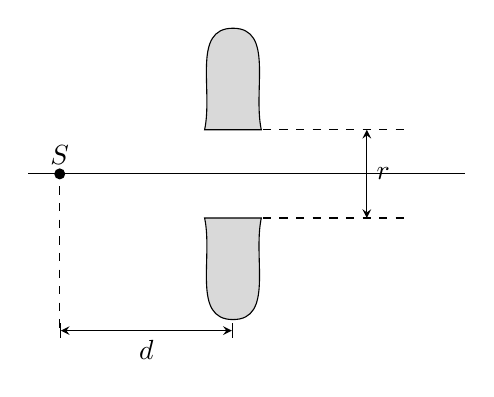
\begin{tikzpicture}[>=stealth]

\draw (-2.6,0)--(2.95,0);\fill (-2.2,0)circle(.07)node[above]{$S$};
\draw[fill=gray!30] (-.36,.56) to[out=78,in=180] (0,1.85) to[out=0,in=102] (.36,.56)--cycle;
\draw[fill=gray!30] (-.36,-.56) to[out=-78,in=180] (0,-1.85) to[out=0,in=-102] (.36,-.56)--cycle;
\draw[dashed](.38,.56)--(2.24,.56) (.38,-.56)--(2.24,-.56);
\draw[<->](1.7,-.56)--(1.7,.56) node[midway,right]{$r$};
\draw[|<->|](-2.2,-1.99)--(0,-1.99)node[midway,below]{$d$};\draw[dashed](-2.2,-.16)--(-2.2,-1.99);
\end{tikzpicture}\end{center}
Точечный источник света находится на главной оптической оси тонкой собирающей линзы. Линзу разрезали на две половины, которые раздвинули на расстояние r  =  $2\,\text{мм}$ (см. рис.). Сделайте рисунок с указанием хода лучей через данную систему. Найдите расстояние от точечного источника света до линзы, если расстояние между действительными изображениями источника l  =  $6\,\text{мм}$. Фокусное расстояние линзы F  =  $40\,\text{см}$.
}{
\smallskip\noindent\textbf{Решение}\par
После того, как линзу разрезали пополам и раздвинули, получилась система из двух линз, у каждой из которой главная оптическая ось поднялась на величину $\frac{r}{2} .$ Построим изображение источника тока через каждую из линз:

\begin{center}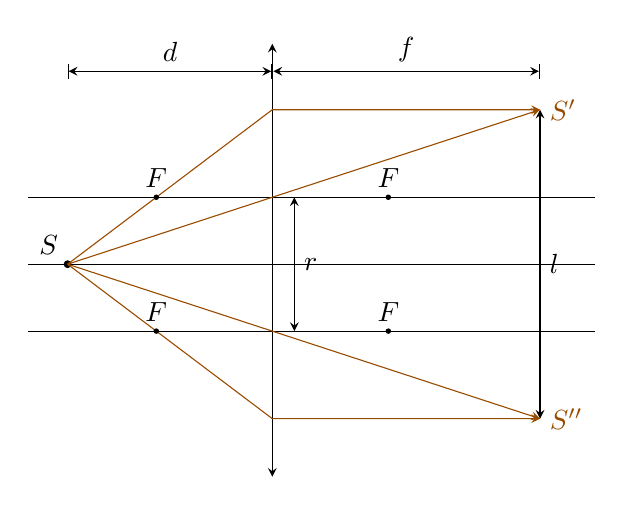
\begin{tikzpicture}[>=stealth]

\draw(-3.1,0)--(4.1,0) (-3.1,.85)--(4.1,.85) (-3.1,-.85)--(4.1,-.85);
\draw[<->](0,-2.7)--(0,2.8);\fill(-2.6,0)circle(.05)node[above left]{$S$};
\draw[orange!60!black,->](-2.6,0)--(0,1.962)--(3.4,1.962)node[right]{$S'$};
\draw[orange!60!black,->](-2.6,0)--(3.4,1.962);
\draw[orange!60!black,->](-2.6,0)--(0,-1.962)--(3.4,-1.962)node[right]{$S''$};
\draw[orange!60!black,->](-2.6,0)--(3.4,-1.962);
\foreach \y in {-.85,.85}{\fill(-1.4733,\y)circle(.035)node[above]{$F$} (1.4733,\y)circle(.035)node[above]{$F$};}
\draw[<->](.28,-.85)--(.28,.85)node[midway,right]{$r$};
\draw[<->](3.4,-1.962)--(3.4,1.962)node[midway,right]{$l$};
\draw[|<->|](-2.6,2.45)--(0,2.45)node[midway,above]{$d$};
\draw[|<->|](0,2.45)--(3.4,2.45)node[midway,above]{$f$};
\end{tikzpicture}\end{center}


\begin{center}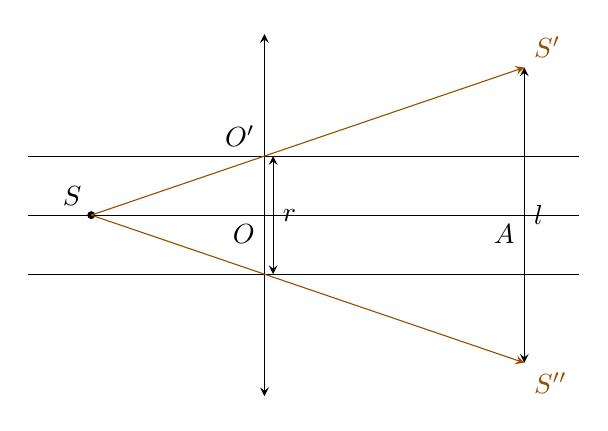
\begin{tikzpicture}[>=stealth]

\draw (-3,0)--(4,0) (-3,.75)--(4,.75) (-3,-.75)--(4,-.75);\draw[<->](0,-2.3)--(0,2.3);
\fill(-2.2,0)circle(.05)node[above left]{$S$};\node[below left]at(0,0){$O$};\node[above left]at(0,.75){$O'$};
\draw[orange!60!black,->](-2.2,0)--(3.3,1.875)node[above right]{$S'$};
\draw[orange!60!black,->](-2.2,0)--(3.3,-1.875)node[below right]{$S''$};
\draw[<->](3.3,-1.875)--(3.3,1.875)node[midway,right]{$l$};\node[below left]at(3.3,0){$A$};
\draw[<->](.11,-.75)--(.11,.75)node[midway,right]{$r$};
\end{tikzpicture}\end{center}


Из подобия треугольников $SOO'$ и $SS'S''$ следует, что $\frac{r}{d} = \frac{l}{d + f} ,$ где f  — расстояние от линзы до изображения. Запишем формулу тонкой собирающей линзы $\frac{1}{d} + \frac{1}{f} = \frac{1}{F} .$ Объединяя формулы, получаем:

\[\frac{1}{d} + \frac{r}{d ( L - r )} = \frac{1}{F} .\]

Выразим расстояние от источника света до линзы:

\[d = \frac{LF}{L - r} = \frac{6 \cdot 40}{6 - 2} = 60 \,\text{см}.\]

Ответ: $60\,\text{см}$.
}

% Source 35184: https://phys-ege.sdamgia.ru/problem?id=35184
\BankTask{35184}{
\begin{center}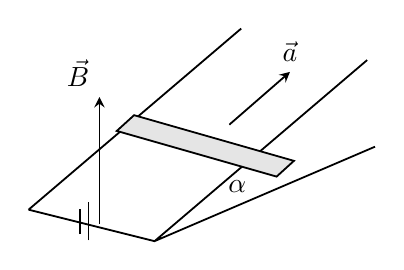
\begin{tikzpicture}[>=stealth,line width=.65pt]\draw (0,0)--(1.6,-.4)--(4.3,1.9) (0,0)--(2.7,2.3) (1.6,-.4)--(4.4,.8);\draw[fill=gray!20] (1.12,1)--(3.15,.42)--(3.37,.62)--(1.34,1.2)--cycle;\draw[->] (.9,-.18)--(.9,1.43) node[above left]{$\vec B$};\draw[->] (2.55,1.08)--(3.32,1.75) node[above]{$\vec a$};\draw (.65,-.31)--(.65,.01) (.76,-.39)--(.76,.1);\node at (2.65,.3){$\alpha$};\end{tikzpicture}\end{center}

 Горизонтальный проводящий стержень прямоугольного сечения поступательно движется с ускорением вверх по гладкой наклонной плоскости в вертикальном однородном магнитном поле (см. рис.). По стержню протекает ток $I=4\,\text{А}.$ Угол наклона плоскости $\alpha =30 ^\circ.$ Отношение массы стержня к его длине $\frac{m}{L} =0{,}1\,\text{кг/м}.$ Модуль индукции магнитного поля $B=0{,}2\,\text{Тл}.$ Чему равно ускорение стержня?
}{
\smallskip\noindent\textbf{Решение}\par
\begin{center}\begin{tikzpicture}[>=stealth,line width=.65pt]\draw (0,0)--(4,0) (0,0)--(3.4,1.95);\draw (.48,0) arc (0:30:.48) node[right]{$\alpha$};\draw[fill=gray!20,rotate=30] (1.45,0) rectangle (2.45,.55);\coordinate (o) at (1.55,1.2);\draw[->](o)--++(2.25,1.3)node[above]{$x$};\draw[->](o)--++(-1.1,1.9)node[left]{$y$};\draw[->,thick](o)--++(-.5,.87)node[below left]{$\vec N$};\draw[->,thick](o)--++(1.5,0)node[right]{$\vec F_{\text{А}}$};\draw[->,thick](o)--++(0,-1)node[below]{$m\vec g$};\draw (2.12,1.2) arc (0:30:.57);\node at (2.28,1.38){$\alpha$};\draw (1.55,.58) arc (-90:-60:.62);\node at (1.89,.5){$\alpha$};\end{tikzpicture}\end{center}

На стержень действуют сила тяжести mg, сила Ампера $F_{A}$ и сила реакции опоры N. Изобразим эти силы на рисунке.
По второму закону Ньютона $m\vec{g} + \vec{N} + \vec F_A=m\vec{a}.$
В проекции на выбранную ось Oх:

\[F_A \cos \alpha - mg \sin \alpha =ma.\]

Сила Ампера находится по формуле $F_A = BIl \sin \beta ,$ где $\beta$  =  $90$\ensuremath{{}^{\circ}}  — угол между направлением тока и вектором магнитной индукции.
Тогда получаем:

\[ma + mg \sin \alpha = BIl \cos \alpha .\]

Отсюда ускорение стержня равно:

\[a= \frac{BIl \cos \alpha}{m} - g \sin \alpha = \frac{0{,}2 \cdot 4 \cdot \cos 30 ^\circ}{0{,}1} - 10 \cdot 0{,}5\approx 1{,}9 \,\text{м/с} ^2 .\]

Ответ: $1{,}9\,\text{м/с}^{2}$.
}

% Source 50813: https://phys-ege.sdamgia.ru/problem?id=50813
\BankTask{50813}{
Линза, фокусное расстояние которой $30\,\text{см}$, даёт на экране резкое изображение предмета c пятикратным увеличением. Экран пододвинули к линзе вдоль её главной оптической оси. Затем при неизменном положении линзы передвинули предмет на $3\,\text{см}$ так, чтобы изображение снова стало резким. На какое расстояние сдвинули экран относительно его первоначального положения? Сделайте рисунок построения изображений в линзе с указанием хода лучей.
}{
\smallskip\noindent\textbf{Решение}\par
Построим изображение предмета в собирающей линзе в первом случае:


\begin{center}\begin{tikzpicture}[>=stealth,line width=.65pt]\draw (-2.1,0)--(7.95,0);\draw[<->](0,-2.55)--(0,2.55);\draw[cyan!50,line width=2.5pt](7.5,-2.48)--(7.5,2.46);\node[below]at(7.5,-2.5){Экран};\draw[->,orange!80!black](-1.5,0)node[below left]{$B$}--(-1.5,.35)node[above left]{$A$};\draw[->,red!70!black](7.5,0)node[below left]{$C$}--(7.5,-1.75)node[below left]{$D$};\draw[green!55!black](-1.5,.35)--(0,.35)--(7.5,-1.75) (-1.5,.35)--(7.5,-1.75);\draw[->,green!55!black](-1,.35)--(-.64,.35);\draw[->,green!55!black](1.8,{-.35*1.8/1.5})--(2.14,{-.35*2.14/1.5});\draw[->,green!55!black](2.65,{.35-.28*2.65})--(3,{.35-.28*3});\fill(-1.25,0)circle(.026)node[below right]{$F$};\fill(1.25,0)circle(.026)node[above]{$F$};\node[below left]at(0,0){$O$};\draw[thin](-1.5,.38)--(-1.5,2.15);\draw[<->](-1.5,2.1)--(0,2.1)node[midway,above]{$d_1$};\draw[<->](0,2.1)--(7.5,2.1)node[midway,above]{$f_1$};\end{tikzpicture}\end{center}


Используем формулы тонкой линзы $\frac{1}{d_1} + \frac{1}{f_1} = \frac{1}{F}$ и увеличения, даваемого собирающей линзой, $\Gamma = \frac{f_1}{d_1} .$ Из них находим расстояние от предмета до линзы и от изображения до линзы: $d_1 = 1{,}2F,$ $f_1 = 6F.$
Построим изображение предмета в собирающей линзе во втором случае:


\begin{center}\begin{tikzpicture}[>=stealth,line width=.65pt]\draw (-2.1,0)--(7.95,0);\draw[<->](0,-2.55)--(0,2.55);\draw[cyan!50,line width=2.5pt](5.4167,-2.48)--(5.4167,2.46);\node[below]at(5.4167,-2.5){Экран};\draw[->,orange!80!black](-1.625,0)node[below left]{$B$}--(-1.625,.35)node[above left]{$A$};\draw[->,red!70!black](5.4167,0)node[below left]{$C_1$}--(5.4167,-1.166673846153846)node[below left]{$D_1$};\draw[green!55!black](-1.625,.35)--(0,.35)--(5.4167,-1.166673846153846) (-1.625,.35)--(5.4167,-1.166673846153846);\draw[->,green!55!black](-1,.35)--(-.64,.35);\draw[->,green!55!black](1.8,{-.35*1.8/1.625})--(2.14,{-.35*2.14/1.625});\draw[->,green!55!black](2.65,{.35-.28*2.65})--(3,{.35-.28*3});\fill(-1.25,0)circle(.026)node[below right]{$F$};\fill(1.25,0)circle(.026)node[above]{$F$};\node[below left]at(0,0){$O$};\draw[thin](-1.625,.38)--(-1.625,2.15);\draw[<->](-1.625,2.1)--(0,2.1)node[midway,above]{$d_2$};\draw[<->](0,2.1)--(5.4167,2.1)node[midway,above]{$f_2$};\draw[dashed](-1.5,0)--(-1.5,2.15) (7.5,-2.3)--(7.5,2.22);\draw[<->](-1.5,1.68)--(-1.625,1.68)node[midway,left=.24cm]{$\Delta d$};\draw[<->](5.4167,2.1)--(7.5,2.1)node[midway,above]{$x$};\end{tikzpicture}\end{center}


При этом видно, что если по условию расстояние от линзы до экрана уменьшили на величину x, то расстояние от предмета до линзы увеличилось на величину $\Delta d.$ Запишем формулу собирающей линзы для этого случая:

$\frac{1}{d_2} + \frac{1}{f_2} = \frac{1}{F} ,$
$\frac{1}{d_1 + \Delta d} + \frac{1}{f_1 - x} = \frac{1}{F} ,$
$\frac{1}{1{,}2F + \Delta d} + \frac{1}{6F - x} = \frac{1}{F} ,$

откуда находим искомое расстояние:

\[x = \frac{5F \Delta d}{0{,}2F + \Delta d} = \frac{5 \cdot 30 \cdot 3}{0{,}2 \cdot 30 + 3} = 50 \,\text{см}.\]

Ответ: $50\,\text{см}$.
}

% Source 32269: https://phys-ege.sdamgia.ru/problem?id=32269
\BankTask{32269}{
\begin{center}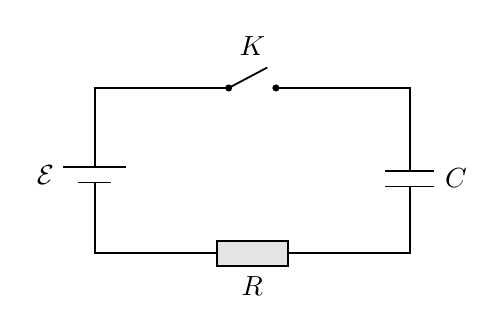
\begin{tikzpicture}[>=stealth,line width=.65pt]\draw (0,1.1)--(0,2.1)--(1.7,2.1) (2.3,2.1)--(4,2.1)--(4,1.05) (4,.85)--(4,0)--(2.45,0) (1.55,0)--(0,0)--(0,.9);\draw (-.4,1.1)--(.4,1.1) (-.21,.9)--(.21,.9) (3.69,1.05)--(4.31,1.05) (3.69,.85)--(4.31,.85);\draw (1.7,2.1)--(2.19,2.36);\foreach \x in {1.7,2.3}{\fill (\x,2.1) circle (.045);}\draw[fill=gray!20](1.55,-.16)rectangle(2.45,.16);\node[left]at(-.39,1){$\mathcal E$};\node[right]at(4.32,.95){$C$};\node[below]at(2,-.17){$R$};\node[above]at(2,2.38){$K$};\end{tikzpicture}\end{center}

Незаряженный конденсатор с емкостью C  =  $0{,}1$ мкФ подключают к источнику тока по схеме, показанной на рисунке. Сопротивление резистора R  =  $500\,\text{Ом}$, сопротивлением проводов и внутренним сопротивлением источника можно пренебречь. После замыкания ключа К на резисторе выделяется тепло равное $7{,}2$ мкДж. Чему равно ЭДС источника?
}{
\smallskip\noindent\textbf{Решение}\par
При замыкании цепи через резистор проходит ток зарядки до тех, пока конденсатор не зарядится до напряжения, равного ЭДС источника тока.
При этом через источник тока протечет заряд, равный $q=CU=C \mathcal{E} .$ Тогда в источнике тока будет совершена работа $A=q \mathcal{E} =C \mathcal{E} ^2 .$
Энергия, которую приобретет при этом заряженный конденсатор, равна:

\[W_{\,\text{р}}= \frac{CU ^2}{2} = \frac{C \mathcal{E} ^2}{2} .\]

Поскольку сопротивлением проводов и внутренним сопротивлением источника тока можно пренебречь, то можно применить закон сохранения энергии:

$A_{\,\text{ист}}=Q + W_p,$
$C \mathcal{E} ^2 =Q + \frac{C \mathcal{E} ^2}{2} ,$

 откуда:

\[\mathcal E=\sqrt{\frac{2Q}{C}}=\sqrt{\frac{2\cdot7{,}2\cdot10^{-6}}{0{,}1\cdot10^{-6}}}=12\,\text{В}.\]

Ответ: $12\,\text{В}$.
}

% Source 7902: https://phys-ege.sdamgia.ru/problem?id=7902
\BankTask{7902}{
\begin{center}\begin{tikzpicture}[>=stealth,line width=.65pt]\draw (-4.65,0)--(3.4,0) (-2,-1.95)--(-2,1.95) (0,-1.95)--(0,1.95);\node[above]at(-2,1.95){Э};\node[above]at(0,1.95){Л};\fill (-4.3,.85)circle(.055)node[above left]{$S$};\draw[thin](-4.3,0)--(-4.3,.85)node[midway,left]{$H$};\node[below]at(-3.1,0){$b$};\fill (-2,-.68)circle(.035)node[left]{$A$};\node[right]at(-2,-.36){$h$};\node[above right]at(-2,0){$F$};\fill (2,0)circle(.045)node[above]{$F$};\end{tikzpicture}\end{center}

На расстоянии b = $40\,\text{см}$ от собирающей линзы с фокусным расстоянием $20\,\text{см}$ находится точечный источник света, расположенный на высоте Н = $5\,\text{см}$ от главной оптической оси. В левой фокальной плоскости линзы расположен тонкий экран с малым отверстием  А, находящемся в плоскости рисунка на расстоянии h = $4\,\text{см}$ от главной оптической оси. Изобразите ход луча SA и определите, на каком расстоянии х от плоскости линзы этот луч  от точечного источника, пройдя через отверстие в экране и линзу, пересечет главную оптическую ось. Дифракцией пренебречь.
}{
\smallskip\noindent\textbf{Решение}\par
\begin{center}\begin{tikzpicture}[>=stealth,line width=.65pt]\draw (-4.65,0)--(7,0) (-2,-2.3)--(-2,1.8) (0,-2.3)--(0,1.8);\node[above]at(-2,1.8){Э};\node[above]at(0,1.8){Л};\draw[thin](-4,0)--(-4,.8)node[midway,left]{$H$} (4,0)--(4,-.8)node[midway,above left]{$H\prime$};\draw[blue!70!black] (-4,.8)--(0,.8)--(6.7,-1.88) (-4,.8)--(6.7,-1.34);\draw[green!45!black] (-4,.8)--(0,-2.08)--(7,.16);\draw[->,blue!70!black](-1,.8)--(-.8,.8) (1.1,.36)--(1.3,.28) (.9,-.18)--(1.1,-.22);\draw[->,green!45!black](1.1,-1.728)--(1.3,-1.664);\fill(-4,.8)circle(.045)node[above left]{$S$};\fill(4,-.8)circle(.045)node[below left]{$S\prime$};\fill(-2,-.64)circle(.04)node[below left]{$A$};\node[above right]at(-2,0){$F$};\node[right]at(-2,-.33){$h$};\node[below]at(-3,0){$b$};\fill(2,0)circle(.045)node[above]{$F$};\end{tikzpicture}\end{center}

Построим изображение источника $S',$ используя свойства тонкой линзы: луч, идущий параллельно оптической оси, после преломления в линзе проходит через ее фокус; луч, идущий через середину линзы, не преломляется. Луч SA после преломления в линзе также пройдет через точку $S'$ (см. рис.).
Теперь вычислим, где он пересекает оптическую ось. Луч преломляется в линзе на расстоянии y от оптической оси. Из подобия треугольников находим, что

\[\frac{H + h}{b - F} = \frac{y - h}{F} \Longleftrightarrow y= \frac{F ( H + h )}{b - F} + h= \frac{bh + HF}{b - F} .\]

Из точки А проведем луч через оптический центр линзы О, который не преломляется. Точка А является побочным фокусом линзы, поэтому этот луч параллелен преломленному лучу.
Из подобия треугольников находим, что

$\frac{h}{F} = \frac{y}{x}$
$x=y \cdot \frac{F}{h} = \frac{F}{h} \cdot \frac{bh + HF}{b - F} = \frac{20}{4} \cdot \frac{4 \cdot 40 + 20 \cdot 5}{40 - 20} =65\,\text{см}$

Ответ: ход луча изображен на рисунке, $x=65\,\text{см}.$
}

% Source 26734: https://phys-ege.sdamgia.ru/problem?id=26734
\BankTask{26734}{
Два точечных источника света находятся на главной оптической оси тонкой собирающей линзы на расстоянии L  =  $1\,\text{м}$ друг от друга. Линза находится между ними. Расстояние от линзы до одного из источников x  =  $20\,\text{см}$. Изображения обоих источников получились в одной точке. Найдите оптическую силу линзы. Постройте на отдельных рисунках изображения двух источников в линзе, указав ход лучей.
}{
\smallskip\noindent\textbf{Решение}\par
$1$.  Так как источники находятся с разных сторон от линзы, то для одного из них изображение должно быть действительным, а для другого  — мнимым (см. рис.).
$2$.  Источник, который находится ближе к линзе, дает мнимое изображение.


\begin{center}\begin{tikzpicture}[>=stealth,line width=.65pt]\draw(-4.3,0)--(3.1,0);\draw[<->](0,-2.55)--(0,2.35)node[left]{Л};\draw[orange!80!black] (-3,0)--(2,1.72) (-1.25,0)--(0,1.03)--(2,1.72) (-1.25,-1.03)--(2.25,1.84);\draw[dashed](2,0)--(2,2.18);\fill(-3,0)circle(.045)node[below left]{$S_1^{\prime}$};\fill(-1.25,0)circle(.045)node[below left]{$S_1$};\fill(-2,0)circle(.045)node[below]{$F$};\fill(2,0)circle(.045)node[below]{$F$};\draw[thin](-3,0)--(-3,-2.35) (-1.25,0)--(-1.25,-1.85);\draw[<->](-3,-2.35)--(0,-2.35)node[midway,above]{$f$};\draw[<->](-1.25,-1.8)--(0,-1.8)node[midway,above]{$x$};\draw[->,orange!80!black](1.4,1.515)--(1.7,1.62) (-.75,.412)--(-.5,.618);\end{tikzpicture}\end{center}


 Источник, который находится дальше от линзы, дает действительное изображение.


\begin{center}\begin{tikzpicture}[>=stealth,line width=.65pt]\draw(-3.25,0)--(4,0);\draw[<->](0,-2.55)--(0,2.35)node[left]{Л};\draw[orange!80!black](3.15,0)--(0,1.38)--(-2,0) (3.15,-1.38)--(-2,1);\draw[dashed](-1.25,0)--(-1.25,2.2);\fill(-2,0)circle(.045)node[below left]{$S_2^{\prime}$};\fill(3.15,0)circle(.045)node[below right]{$S_2$};\fill(-1.25,0)circle(.045)node[below]{$F$};\draw[thin](-2,0)--(-2,-2.35) (3.15,0)--(3.15,-2.35);\draw[<->](-2,-2.35)--(0,-2.35)node[midway,above]{$f$};\draw[<->](0,-2.35)--(3.15,-2.35)node[midway,above]{$L-x$};\draw[->,orange!80!black](1.2,.855)--(.9,.986) (-.8,.83)--(-1,.69);\end{tikzpicture}\end{center}


$3$.  Формулы тонкой линзы для двух источников имеют вид:

$\frac{1}{x} - \frac{1}{f} = \frac{1}{F}$ (минус перед f, так как изображение мнимое), ($1$)
$\frac{1}{L - x} + \frac{1}{f} = \frac{1}{F} ,$ ($2$)

 где F  — фокусное расстояние линзы, f  — расстояние от линзы до точки, в которой находятся оба изображения.
$4$.  Решая систему уравнений ($1$)-($2$), получим:

\[F= \frac{2x ( L - x )}{L} .\]

$5$.  Так как оптическая сила линзы $D= \frac{1}{F} ,$ то получим:

\[D= \frac{L}{2x ( L - x )} = \frac{1}{2 \cdot 0{,}2 ( 1 - 0{,}2 )} =3{,}125 \,\text{дптр}.\]

Ответ: D  =  $3{,}125\,\text{дптр}$.
}

% Source 19879: https://phys-ege.sdamgia.ru/problem?id=19879
\BankTask{19879}{
\begin{center}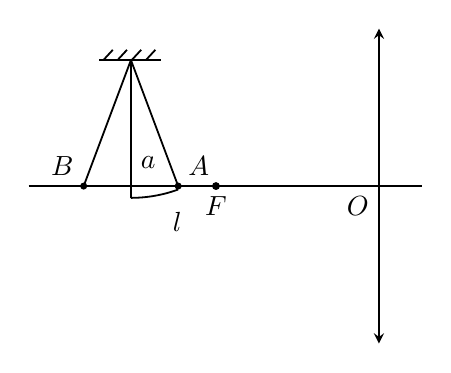
\begin{tikzpicture}[>=stealth,line width=.65pt]\draw(-4,0)--(1,0);\draw[<->](.45,-2)--(.45,2);\draw(-2.7,1.6)--(-3.3,0) (-2.7,1.6)--(-2.1,0) (-2.7,1.6)--(-2.7,-.15);\draw (-2.7,-.15) arc (-90:-70:1.75);\draw(-3.1,1.6)--(-2.32,1.6);\foreach \x in {-3.05,-2.87,...,-2.33} {\draw (\x,1.6)--++(.12,.13);}\fill(-3.3,0)circle(.045)node[above left]{$B$};\fill(-2.1,0)circle(.045)node[above right]{$A$};\fill(-1.62,0)circle(.05)node[below]{$F$};\node[below left]at(.45,0){$O$};\node at(-2.48,.3){$a$};\node at(-2.11,-.45){$l$};\end{tikzpicture}\end{center}

Шарик подвешен на нити и совершает колебания. Его крайние точки, А и B, лежат на оптической оси собирающей линзы силой D  =  $50\,\text{дптр}$. Проекция точки равновесия шарика находится на расстоянии $\sqrt{5}$ см от первого фокуса линзы. Расстояние от нее до крайних точек равно $1\,\text{см}$. Найдите расстояние между изображениями крайних точек A и B в собирающей линзе.
}{
\smallskip\noindent\textbf{Решение}\par
\begin{center}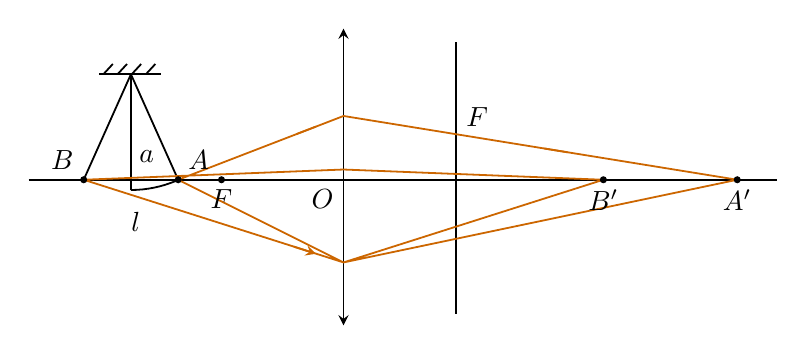
\begin{tikzpicture}[>=stealth,line width=.65pt]\draw(-4,0)--(5.5,0);\draw[<->](0,-1.85)--(0,1.92);\draw(1.43,-1.7)--(1.43,1.75);\draw(-2.7,1.34)--(-3.3,0) (-2.7,1.34)--(-2.1,0) (-2.7,1.34)--(-2.7,-.13);\draw(-2.7,-.13)arc(-90:-67:1.47);\draw(-3.1,1.34)--(-2.32,1.34);\foreach \x in {-3.05,-2.87,...,-2.33} {\draw (\x,1.34)--++(.12,.13);}\draw[orange!80!black](-2.1,0)--(0,.81)--(5,0) (-2.1,0)--(0,-1.05)--(5,0) (-3.3,0)--(0,.13)--(3.3,0) (-3.3,0)--(0,-1.05)--(3.3,0);\draw[->,orange!80!black](-.6,.579)--(-.35,.675) (2.55,.397)--(2.85,.348) (-.63,-.85)--(-.35,-.94);\fill(-3.3,0)circle(.045)node[above left]{$B$};\fill(-2.1,0)circle(.045)node[above right]{$A$};\fill(3.3,0)circle(.045)node[below]{$B^{\prime}$};\fill(5,0)circle(.045)node[below]{$A^{\prime}$};\fill(-1.55,0)circle(.045)node[below]{$F$};\node[above right]at(1.43,.55){$F$};\node[below left]at(0,0){$O$};\node at(-2.5,.3){$a$};\node at(-2.64,-.54){$l$};\end{tikzpicture}\end{center}

Запишем уравнения для тонкой линзы: $\frac{1}{F} = \frac{1}{OB} + \frac{1}{OB'} ;$ $\frac{1}{F} = \frac{1}{OA} + \frac{1}{OA'} .$ По определению $D= \frac{1}{F} ,$ следовательно, $F= \frac{1}{D} =2 \,\text{см}.$ Откуда

$OA=F + l - A=2 + \sqrt{5} - 1=1 + \sqrt{5} \,\text{см},$ 
$OB=F + l + A=3 + \sqrt{5} \,\text{см}.$

Тогда 

$\frac{1}{OB'} = \frac{1}{F} - \frac{1}{OB} =50 - \frac{1}{( 3 + \sqrt{5} ) \cdot 0{,}01} =25 ( \sqrt{5} - 1 ) ;$
$OB'= \frac{1}{25 ( \sqrt{5} - 1 )} = \frac{\sqrt{5} + 1}{100} \,\text{м};$
$\frac{1}{OA'} = \frac{1}{F} - \frac{1}{OA} =50 - \frac{1}{( 1 + \sqrt{5} ) \cdot 0{,}01} =25 ( 3 - \sqrt{5} ) ;$
$OA'= \frac{1}{25 ( 3 - \sqrt{5} )} = \frac{3 + \sqrt{5}}{100} \,\text{м};$
$|OA' - OB'|=| \frac{\sqrt{5} + 1 - 3 - \sqrt{5}}{100} |= \frac{1}{50} \,\text{м} = 2\,\text{см}.$

Ответ: $|OA' - OB'|=2\,\text{см}.$
}

% Source 3022: https://phys-ege.sdamgia.ru/problem?id=3022
\BankTask{3022}{
Бассейн глубиной $3\,\text{м}$ заполнен водой, относительный показатель преломления на границе воздух  — вода $1{,}33$. Каков радиус светового круга на поверхности воды от электрической лампы на дне бассейна?
}{
\smallskip\noindent\textbf{Решение}\par
\begin{center}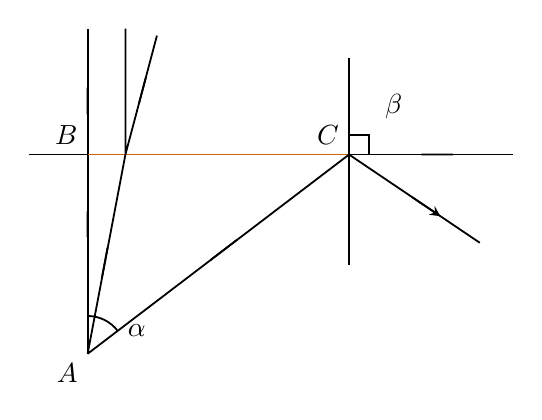
\begin{tikzpicture}[>=stealth,line width=.65pt]\draw(-.75,0)--(5.4,0);\draw (0,-2.53)--(0,1.6) (3.32,-1.4)--(3.32,1.22);\coordinate (A) at (0,-2.53);\coordinate (C) at (3.32,0);\draw[orange!80!black](0,0)--(C);\draw (A)--(C)--(4.98,-1.12) (A)--(.48,0)--(.48,1.6) (A)--(.48,0)--(.88,1.51);\draw[->](0,.51)--(0,.85) (0,-1.05)--(0,-.72) (.18,-1.57)--(.253,-1.18) (.65,.64)--(.74,.98) (1.56,-1.34)--(1.9,-1.08) (4.24,0)--(4.64,0) (4.12,-.54)--(4.48,-.783);\draw (0,-2.05)arc(90:37.3:.48)node[right]{$\alpha$};\draw (3.32,.25)--(3.57,.25)--(3.57,0);\node[above right]at(3.65,.32){$\beta$};\node[below left]at(A){$A$};\node[above left]at(0,0){$B$};\node[above left]at(C){$C$};\end{tikzpicture}\end{center}

Рассмотрим ход лучей, исходящих из точки А на дне бассейна. Вертикальный луч АВ не изменяет своего направления после прохождения границы раздела, все остальные лучи испытывают преломление или отражаются от границы раздела.
Полное внутреннее отражение происходит начиная с такого значения угла падения $\alpha ,$ при котором угол преломления $\beta$ равен $90 ^\circ.$ Следовательно, предельное значение угла $\alpha ,$ при котором свет выходит из воды, определяется условием $\sin \alpha = \frac{1}{n} .$
Из треугольника АВС найдем радиус светового круга ВС:

\[BC=AB \cdot \tan \alpha = \frac{AB}{\sqrt{n ^2 - 1}} = \frac{3 \,\text{м}}{\sqrt{1{,}33 ^2 - 1}} \approx 3{,}4\,\text{м}.\]

Ответ: $3{,}4\,\text{м}$.
}

% Source 5177: https://phys-ege.sdamgia.ru/problem?id=5177
\BankTask{5177}{
\begin{center}\begin{tikzpicture}[>=stealth,line width=.65pt]\draw(-3.75,0)--(2.95,0);\draw[<->](0,-1.95)--(0,1.95);\draw[orange!80!black](-3.4,0)--(-2.3,1.1)--(-2.3,0)--cycle;\foreach \x/\l in {-3.4/2F,-1.7/F,1.7/F}{\fill (\x,0)circle(.035)node[below]{$\l$};}\node[above left]at(-3.4,0){$A$};\node[above left]at(-2.3,1.1){$B$};\node[above right]at(-2.3,0){$C$};\end{tikzpicture}\end{center}

 Равнобедренный	прямоугольный треугольник ABC расположен перед тонкой собирающей линзой оптической силой $2{,}5\,\text{дптр}$ так, что его катет АС лежит на главной оптической оси линзы (см. рисунок). Вершина прямого угла С лежит ближе к центру линзы, чем вершина острого угла А. Расстояние от центра линзы до точки А равно удвоенному фокусному расстоянию линзы, АС = $4\,\text{см}$. Постройте изображение треугольника и найдите площадь получившейся фигуры.
}{
\smallskip\noindent\textbf{Решение}\par
Изображение треугольника построено на рисунке. 


\begin{center}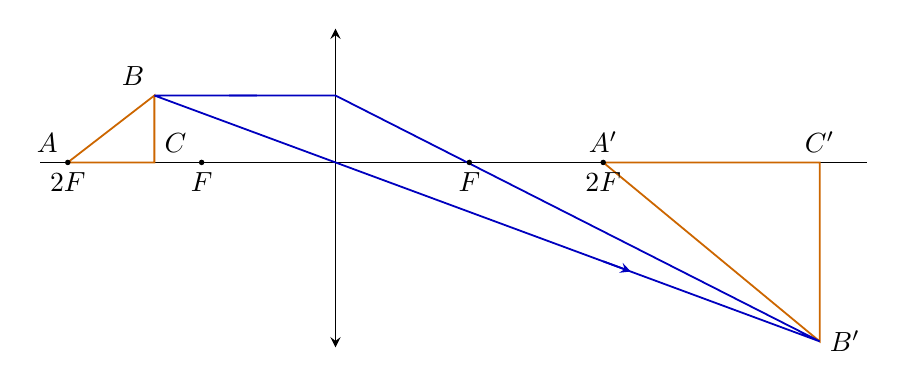
\begin{tikzpicture}[>=stealth,line width=.65pt]\draw(-3.75,0)--(6.75,0);\draw[<->](0,-2.35)--(0,1.7);\draw[orange!80!black](-3.4,0)--(-2.3,.85)--(-2.3,0)--cycle (3.4,0)--(6.15,-2.273)--(6.15,0)--cycle;\draw[blue!75!black](-2.3,.85)--(0,.85)--(6.15,-2.273) (-2.3,.85)--(6.15,-2.273);\draw[->,blue!75!black](-1.35,.85)--(-1,.85) (3.4,-1.256)--(3.75,-1.385);\foreach \x/\l in {-3.4/2F,-1.7/F,1.7/F,3.4/2F}{\fill (\x,0)circle(.035)node[below]{$\l$};}\node[above left]at(-3.4,0){$A$};\node[above left]at(-2.3,.85){$B$};\node[above right]at(-2.3,0){$C$};\node[above]at(3.4,0){$A^{\prime}$};\node[above]at(6.15,0){$C^{\prime}$};\node[right]at(6.15,-2.273){$B^{\prime}$};\end{tikzpicture}\end{center}


Изображение точки B удобно найти как пересечение луча, проходящего через центр линзы и луча, падающего на линзу параллельно главной оптической оси.
Изображение точки С находится в точности под изображением точки В. Положение изображения точки А легко определить из формулы тонкой линзы: 

\[\frac{1}{d} + \frac{1}{f} = \frac{1}{F}\]

Поскольку точка А находится в двойном фокусе, то $d=2F,$ а значит, и $f=2F,$ то есть изображение точки А также находится в двойном фокусе.
Наконец, легко понять, что изображение треугольника вновь будет треугольником. Действительно, если пропустить луч через сторону ВА, то после преломления на этом луче будут находиться изображения всех точек со стороны ВА, то есть гипотенуза прямоугольного треугольника перейдет в гипотенузу треугольника-изображения.

Определим фокусное расстояние

\[F= \frac{1}{D} = \frac{1}{2{,}5\,\text{дптр}} =0{,}4\,\text{м}.\]

Обозначим катет треугольника ABC через $h.$
Найдем расстояние от линзы до изображения точки С ($d=2F - h$):

\[f= \frac{dF}{d - F} = \frac{( 2 \cdot 40 \,\text{см} - 4\,\text{см} ) \cdot 40\,\text{см}}{2 \cdot 40 \,\text{см} - 4\,\text{см} - 40\,\text{см}} \approx 84{,}4\,\text{см}.\]

Горизонтальный катет равен 

\[a=f - 2F\approx 4{,}4\,\text{см}.\]

Из подобия треугольников для вертикального катета треугольника-изображения имеем

\[\frac{h}{b} = \frac{d}{f} \Longleftrightarrow b= \frac{hf}{2F - h} \approx 4{,}4 \,\text{см}.\]

Таким образом, площадь треугольника изображения равна: 

\[S' = \frac{1}{2} ab = \frac{1}{2} ( 4{,}4\,\text{см} ) ^2 \approx 10\,\text{см} ^2 .\]

Ответ: $10\,\text{см} ^2$

Примечание:
В решение можно было использовать тот факт, что треугольник-изображение также является равнобедренным. Это следует из того факта, что луч, проходящий через двойной фокус после преломления в линзе снова попадет в двойной фокус. Тем самым после преломления в линзе луч идет по тем же самым углом к главной оптической оси, что и до преломления в линзе. Поскольку в нашем случае этот угол равен $45 ^\circ,$ то равнобедренный треугольник снова получится равнобедренным.
}

% Source 32270: https://phys-ege.sdamgia.ru/problem?id=32270
\BankTask{32270}{
В колебательном контуре, активное сопротивление которого равно нулю, происходят свободные электромагнитные колебания с периодом T  =  $50{,}24\,\text{мкс}$ и максимальным напряжением на конденсаторе $U_{max}$. Зависимость энергии электрического поля конденсатора от разности потенциалов между его обкладками в пределах от $0$ до $U_{max}$ приведена на графике. Определите максимальное значение силы тока в контуре.

\begin{center}\begin{tikzpicture}[>=stealth,line width=.65pt]\draw[step=.4,gray!50] (0,0)grid(4,4);\draw[->](0,0)--(5.15,0)node[below]{$U$, В};\draw[->](0,0)--(0,4.65)node[left]{$E_{\text{эл}}$, мДж};\node[below left]at(0,0){$0$};\node[left]at(0,2){$0{,}5$};\node[left]at(0,4){$1{,}0$};\node[below]at(2,0){$100$};\node[below]at(4,0){$200$};\draw[orange!80!black,domain=0:4,samples=55]plot(\x,{.2*\x*\x});\fill[orange!80!black](4,3.2)circle(.045);\end{tikzpicture}\end{center}
}{
\smallskip\noindent\textbf{Решение}\par
$1$.  По закону сохранения энергии при отсутствии активного сопротивления в колебательном контуре максимальная энергия заряженного конденсатора равна максимальной энергии магнитного поля катушки с током $W_p=W_{\,\text{м}}.$
При этом максимальная энергия катушки с током равна $W_{\,\text{м}}= \frac{LI ^2 _{\max}}{2} .$
$2$.  В условии задачи известен период колебаний. Период колебаний в колебательном контуре $T=2 \pi \sqrt{LC} .$
$3$.  Максимальная энергия заряженного конденсатора равна $W_{\,\text{р}}= \frac{CU_{\max} ^2}{2} .$
Тогда выражаем:

$C= \frac{2W_{\,\text{р}}}{U_{\max} ^2} ;$
$L= \frac{T ^2}{4 \pi ^2 C} ;$
$I_{\max}= \sqrt{\frac{2W_{\,\text{м}}}{L}} = \frac{4 \pi W_p}{TU_{\max}} .$

Из графика находим, что максимальное значение энергии электрического поля конденсатора $W_p=0{,}8 \cdot 10 ^{ - 3 } \,\text{Дж},$ максимальное напряжение на обкладках конденсатора $U_{\max}=200\,\text{В}.$ При подстановке значений в формулу получаем:

\[I_{\max}= \frac{4 \cdot 3{,}14 \cdot 0{,}8 \cdot 10 ^{ - 3 }}{50{,}24 \cdot 10 ^{ - 6 } \cdot 200} =1\,\text{А}.\]

Ответ: $1\,\text{А}$.
}

% Source 42802: https://phys-ege.sdamgia.ru/problem?id=42802
\BankTask{42802}{
\begin{center}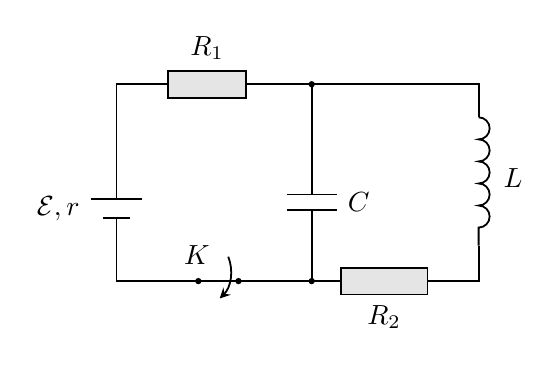
\begin{tikzpicture}[>=stealth,line width=.65pt]\draw (0,1.04)--(0,2.5)--(.65,2.5) (1.65,2.5)--(4.6,2.5)--(4.6,2.08) (4.6,.45)--(4.6,0)--(3.95,0) (2.85,0)--(1.55,0) (1.04,0)--(0,0)--(0,.8);\draw (2.48,2.5)--(2.48,1.1) (2.48,.9)--(2.48,0);\draw (-.32,1.04)--(.32,1.04) (-.17,.8)--(.17,.8) (2.16,1.1)--(2.8,1.1) (2.16,.9)--(2.8,.9);\draw[fill=gray!20](.65,2.33)rectangle(1.65,2.67) (2.85,-.17)rectangle(3.95,.17);\draw (4.6,2.08) arc(90:-90:.14) arc(90:-90:.14) arc(90:-90:.14) arc(90:-90:.14) arc(90:-90:.14) --(4.6,.45);\draw (1.04,0)--(1.55,0);\draw[->] (1.42,.31)arc(22:-45:.49);\foreach \p in {(1.04,0),(1.55,0),(2.48,0),(2.48,2.5)}{\fill \p circle(.04);}\node[left]at(-.34,.92){$\mathcal E,r$};\node[above]at(1.15,2.68){$R_1$};\node[below]at(3.4,-.18){$R_2$};\node[right]at(2.81,1){$C$};\node[right]at(4.79,1.31){$L$};\node[above]at(1.02,.08){$K$};\end{tikzpicture}\end{center}

Электрическая цепь состоит из источника питания с ЭДС $\mathcal{E} = 10\,\text{В}$ и внутренним сопротивлением $r = 1\,\text{Ом},$ двух резисторов с сопротивлениями $R_1 = 5\,\text{Ом}$ и $R_2 = 4\,\text{Ом},$ конденсатора электроёмкостью $C = 80\,\text{мкФ},$ катушки с индуктивностью $L = 200\,\text{мкГн}$ и замкнутого ключа К. Схема этой цепи показана на рисунке. Пренебрегая сопротивлением катушки, определите, какое количество теплоты Q выделится в резисторe $R_2$ в течение длительного времени после размыкания ключа К?
}{
\smallskip\noindent\textbf{Решение}\par
$1$.  До размыкания ключа через катушку течёт постоянный ток, сила которого, по закону Ома для замкнутой цепи, равна 

\[I = \frac{\mathcal{E}}{r + R_1 + R_2} .\]
 При этом напряжение на конденсаторе постоянно и равно падению напряжения на резисторе $R_2,$ поскольку конденсатор и ветвь цепи, содержащая последовательно соединённые резистор $R_2$ и идеальную катушку, соединены параллельно. Поэтому напряжение на конденсаторе равно $U_C = IR_2.$
$2$.  В замкнутом участке цепи, содержащем конденсатор, катушку и резистор $R_2,$ после размыкания ключа возникнут затухающие электромагнитные колебания. Спустя достаточно большое время они прекратятся. В процессе этих колебаний в резисторе $R_2,$ в соответствии с законом Джоуля-Ленца, будет выделяться количество теплоты.
$3$.  Из закона сохранения энергии, примененного для электрической цепи, следует, что к моменту полного затухания указанных колебаний выделившееся в резисторе $R_2$ количество теплоты Q будет равно сумме энергии, запасенной на момент размыкания ключа К в конденсаторе  $W_C= \frac{CU ^2 _C}{2} ,$ и энергии, запасённой в катушке  $W_L= \frac{LI ^2}{2} .$
$4$.  Подставляя в записанные формулы выражения для $U_{C}$ и I, с учётом численных значений физических величин, получим:

$Q=W_C + W_L= \frac{CU ^2 _C}{2} + \frac{LI ^2}{2} = \frac{CR ^2 _2 I ^2}{2} + \frac{LI ^2}{2} = \frac{I ^2 ( CR ^2 _2 + L )}{2} =$

$= \frac{\mathcal{E} ^2 ( CR ^2 _2 + L )}{2 ( r + R_1 + R_2 ) ^2} = \frac{10 ^2 \cdot ( 80 \cdot 10 ^{ - 6 } \cdot 4 ^2 + 200 \cdot 10 ^{ - 6 } )}{2 \cdot ( 1 + 5 + 4 ) ^2} =0{,}74\,\text{мДж}.$

Ответ: $Q= \frac{\mathcal{E} ^2 ( CR ^2 _2 + L )}{2 ( r + R_1 + R_2 ) ^2} =0{,}74\,\text{мДж}.$
}

% Source 41557: https://phys-ege.sdamgia.ru/problem?id=41557
\BankTask{41557}{
\begin{center}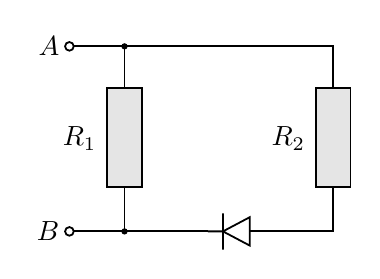
\begin{tikzpicture}[>=stealth,line width=.65pt]\draw (0,2.35)--(3.35,2.35)--(3.35,1.82) (3.35,.56)--(3.35,0)--(2.29,0) (1.76,0)--(0,0) (.7,2.35)--(.7,1.82) (.7,.56)--(.7,0);\draw[fill=gray!20](.48,.56)rectangle(.92,1.82) (3.13,.56)rectangle(3.57,1.82);\draw(2.29,0)--(2.29,.18)--(1.95,0)--(2.29,-.18)--cycle (1.95,.23)--(1.95,-.23) (1.95,0)--(1.76,0);\foreach \p in {(.7,0),(.7,2.35)}{\fill \p circle(.04);}\draw[fill=white](0,0)circle(.055) (0,2.35)circle(.055);\node[left]at(0,2.35){$A$};\node[left]at(0,0){$B$};\node[left]at(.47,1.18){$R_1$};\node[left]at(3.12,1.18){$R_2$};\end{tikzpicture}\end{center}

В цепи, изображённой на рисунке, сопротивление диода в прямом направлении пренебрежимо мало, а в обратном многократно превышает сопротивление резисторов. При подключении к точке A положительного, а к точке B  — отрицательного полюса батареи с ЭДС $6\,\text{В}$ и пренебрежимо малым внутренним сопротивлением потребляемая мощность (тепловая мощность, выделяемая во внешней цепи) равна $13$ Вт. При изменении полярности подключения батареи потребляемая мощность равна $9$ Вт.
Укажите для обоих случаев подключения батареи, протекает ли ток через диод и каждый из резисторов или нет, и определите сопротивления резисторов в этой цепи.
}{
\smallskip\noindent\textbf{Решение}\par
\begin{center}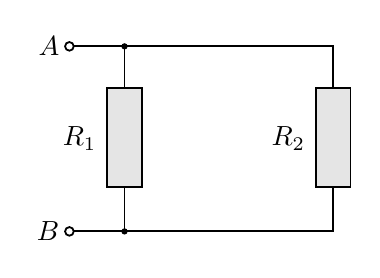
\begin{tikzpicture}[>=stealth,line width=.65pt]\draw (0,2.35)--(3.35,2.35)--(3.35,1.82) (3.35,.56)--(3.35,0)--(0,0) (.7,2.35)--(.7,1.82) (.7,.56)--(.7,0);\draw[fill=gray!20](.48,.56)rectangle(.92,1.82) (3.13,.56)rectangle(3.57,1.82);\foreach \p in {(.7,0),(.7,2.35)}{\fill \p circle(.04);}\draw[fill=white](0,0)circle(.055) (0,2.35)circle(.055);\node[left]at(0,2.35){$A$};\node[left]at(0,0){$B$};\node[left]at(.47,1.18){$R_1$};\node[left]at(3.12,1.18){$R_2$};\end{tikzpicture}\end{center}

 рис. а) 

Если подключить к точке А положительный полюс батареи, а к точке В  — отрицательный, то ток через диод идет. С учетом условия, что в прямом направлении его сопротивление пренебрежимо мало, получаем эквивалентную схему а), в которой два резистора соединены параллельно. Их общее сопротивление находится из формулы 

\[\frac{1}{R} = \frac{1}{R_1} + \frac{1}{R_2} .\]

С учетом, что внутреннее сопротивление батареи пренебрежимо мало, $U= \mathcal{E} ,$ потребляемая мощность равна

\[P_1= \frac{\mathcal{E} ^2}{R} .\]



\begin{center}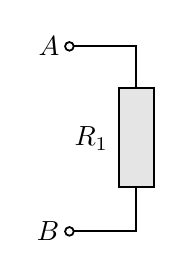
\begin{tikzpicture}[>=stealth,line width=.65pt]\draw (0,2.35)--(.85,2.35)--(.85,1.82) (.85,.56)--(.85,0)--(0,0);\draw[fill=gray!20](.63,.56)rectangle(1.07,1.82);\draw[fill=white](0,0)circle(.055) (0,2.35)circle(.055);\node[left]at(0,2.35){$A$};\node[left]at(0,0){$B$};\node[left]at(.62,1.18){$R_1$};\end{tikzpicture}\end{center}

 рис. б) 

 Если изменить полярность подключения, то ток через диод не пойдет, а, следовательно, не пройдет через резистор $R_{2}$. В этом случае эквивалентная схема будет иметь вид, представленный на рис. б). Мощность тока в этом случае будет равна

\[P_2= \frac{\mathcal{E} ^2}{R_1,}\]

откуда находим сопротивление первого резистора:

\[R_1= \frac{\mathcal{E} ^2}{P_2} = \frac{36}{9} =4\,\text{Ом}.\]

Тогда сопротивление второго резистора равно

\[R_2= \frac{\mathcal{E} ^2}{P_1 - P_2} = \frac{36}{13 - 9} =9\,\text{Ом}.\]

Ответ: $R_1=4\,\text{Ом}; R_2=9\,\text{Ом}.$
}

% Source 29760: https://phys-ege.sdamgia.ru/problem?id=29760
\BankTask{29760}{
Рассеивающая линза с фокусным расстоянием $F_1=10$ см расположена перед собирающей линзой с фокусными расстоянием $F_2=15$ см. Лучи, идущие от точечного источника света, расположенного на расстоянии $d=10$ см от pacceивающей линзы, пройдя систему образовали пучок лучей, параллельный главной оптической оси. Найдите расстояние между линзами.
}{
\smallskip\noindent\textbf{Решение}\par
$1$.  Найдем расстояние от рассеивающей линзы до изображения точечного источника света по формуле тонкой линзы 

\[\frac{1}{d} - \frac{1}{f} = - \frac{1}{F_1} ,\]

 откуда 

\[f= \frac{d F_1}{d + F_1} = \frac{10 \cdot 10}{10 + 10} =5 \,\text{см}.\]

 Это мнимое изображение находится перед рассеивающей линзой. 
$2$.  Учитывая, что данная точка является источником для собирающей линзы, а лучи после прохождения через нее параллельны, делаем вывод, что эта точка находится в фокусе собирающей линзы, то есть на расстоянии $15\,\text{см}$.
$3$.  Тогда расстояние между линзами равно $x=F_2 - f=15 - 5=10 \,\text{см}.$ 

Ответ: $10\,\text{см}$.
}

% Source 30002: https://phys-ege.sdamgia.ru/problem?id=30002
\BankTask{30002}{
\begin{center}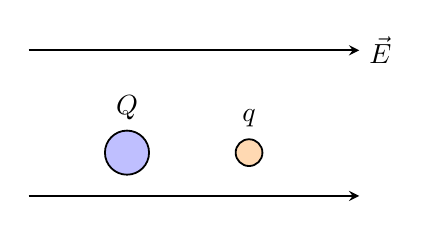
\begin{tikzpicture}[>=stealth,line width=.65pt]\draw[->](0,1.3)--(4.2,1.3)node[right]{$\vec E$};\draw[->](0,-.55)--(4.2,-.55);\draw[fill=blue!25](1.25,0)circle(.28)node[above=.29cm]{$Q$};\draw[fill=orange!30](2.8,0)circle(.17)node[above=.2cm]{$q$};\end{tikzpicture}\end{center}

В однородном электрическом поле с напряженностью E  =  $18\,\text{В}$/м находятся два точечных заряда: Q  =  -$1\,\text{нКл}$ и $q= + 5$ нКл с массами M  =  $5\,\text{г}$ и m  =  $10\,\text{г}$ соответственно (см. рисунок). На каком расстоянии d друг от друга находятся заряды, если их ускорения совпадают по величине и направлению? Сделайте рисунок с указанием всех сил, действующих на заряды. Силой тяжести пренебречь.
}{
\smallskip\noindent\textbf{Решение}\par
\begin{center}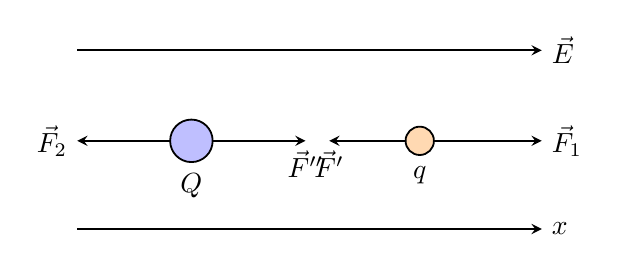
\begin{tikzpicture}[>=stealth,line width=.65pt]\draw[->](0,1.15)--(5.9,1.15)node[right]{$\vec E$};\draw[->](0,-1.12)--(5.9,-1.12)node[right]{$x$};\draw[fill=blue!25](1.45,0)circle(.27)node[below=.29cm]{$Q$};\draw[fill=orange!30](4.35,0)circle(.18)node[below=.2cm]{$q$};\draw[->](1.18,0)--(0,0)node[left]{$\vec F_2$};\draw[->](1.72,0)--(2.9,0)node[below]{$\vec F^{\prime\prime}$};\draw[->](4.17,0)--(3.2,0)node[below]{$\vec F^{\prime}$};\draw[->](4.53,0)--(5.9,0)node[right]{$\vec F_1$};\end{tikzpicture}\end{center}

$1$.  Направим ось Ox по напряженности электрического поля $\vec{E}.$ На заряд q действуют две электрические силы: $F_1=q E$ со стороны однородного поля и сила Кулона $F ^{ \prime } =F= \frac{k q|Q|}{d ^2}$ со стороны другого заряда. На заряд Q действуют сила $F_2=|Q| E$ со стороны однородного поля и сила Кулона $F ^{ \prime \prime } =F= \frac{k q|Q|}{d ^2}$ со стороны заряда q. 
$2$.  В соответствии со вторым законом Ньютона в проекциях на ось Ox имеем: 

$m a=F_1 - F, \qquad ( 1 )$ $M a= - F_2 + F.\qquad ( 2 )$

 Тогда из соотношений ($1$) и ($2$) и условия задачи получим: 

\[\frac{F_1 - F}{m} = \frac{F - F_2}{M} . \qquad ( 3 )\]

$3$.  Подставляя в ($3$) выражения для электрических сил, получим: 

\[d=\sqrt{\frac{kq|Q|(m+M)}{E(m|Q|+qM)}}=\sqrt{\frac{9\cdot10^9\cdot5\cdot10^{-9}\cdot1\cdot10^{-9}\cdot(0{,}01+0{,}005)}{18(0{,}01\cdot1\cdot10^{-9}+0{,}005\cdot5\cdot10^{-9})}}\approx1\,\text{м}.\]

Ответ: $d \approx 1 \,\text{м}.$
}

% Source 20041: https://phys-ege.sdamgia.ru/problem?id=20041
\BankTask{20041}{
\begin{center}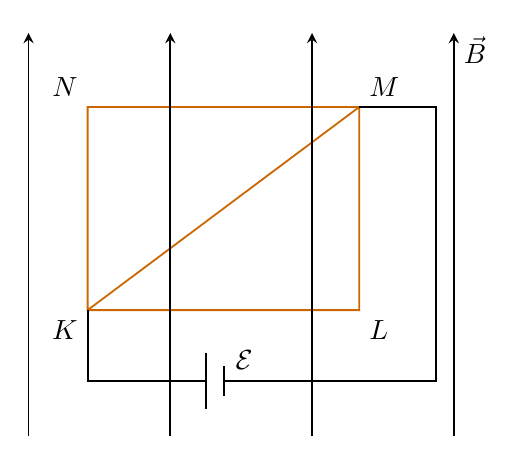
\begin{tikzpicture}[>=stealth,line width=.65pt]\draw[orange!80!black](.75,.9)rectangle(4.2,3.48) (.75,.9)--(4.2,3.48);\draw(.75,.9)--(.75,0)--(2.25,0) (2.48,0)--(5.17,0)--(5.17,3.48)--(4.2,3.48);\draw(2.25,-.35)--(2.25,.35) (2.48,-.19)--(2.48,.19);\node[above right]at(2.5,.02){$\mathcal E$};\foreach \x in {0,1.8,3.6,5.4}{\draw[->](\x,-.7)--(\x,4.42);} \node[below left]at(.75,.9){$K$};\node[above left]at(.75,3.48){$N$};\node[above right]at(4.2,3.48){$M$};\node[below right]at(4.2,.9){$L$};\node[right]at(5.4,4.2){$\vec B$};\end{tikzpicture}\end{center}

Из медной проволоки с удельным сопротивлением $\rho$  =  $1{,}7$ · $10^{-8}$ Ом · м и площадью поперечного сечения S  =  $0{,}2\,\text{мм}^{2}$ изготовлен прямоугольный контур KLMN с диагональю KM (см. рис.). Стороны прямоугольника KL  =  $l_{1}$  =  $20\,\text{см}$ и LM  =  $l_{2}$  =  $15\,\text{см}$. Контур подключили за диагональ к источнику постоянного напряжения с ЭДС $\mathcal{E}$  =  $1{,}4\,\text{В}$ и поместили в однородное магнитное поле с индукцией В  =  $0{,}1$ Тл, параллельной сторонам KN и LM. С какой результирующей силой магнитное поле действует на контур? Сделайте рисунок с указанием сил, действующих на контур. Внутренним сопротивлением источника пренебречь.
}{
\smallskip\noindent\textbf{Решение}\par
\begin{center}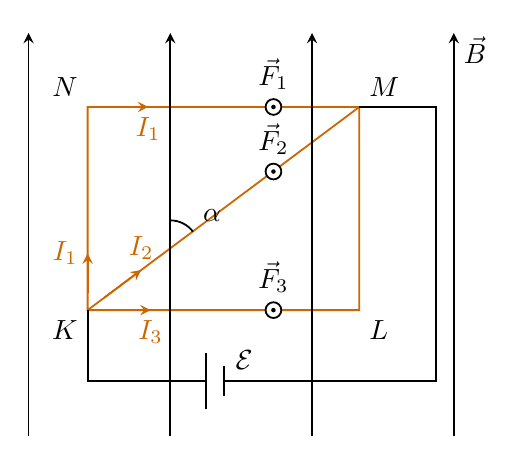
\begin{tikzpicture}[>=stealth,line width=.65pt]\draw[orange!80!black](.75,.9)rectangle(4.2,3.48) (.75,.9)--(4.2,3.48);\draw(.75,.9)--(.75,0)--(2.25,0) (2.48,0)--(5.17,0)--(5.17,3.48)--(4.2,3.48);\draw(2.25,-.35)--(2.25,.35) (2.48,-.19)--(2.48,.19);\node[above right]at(2.5,.02){$\mathcal E$};\foreach \x in {0,1.8,3.6,5.4}{\draw[->](\x,-.7)--(\x,4.42);}\draw[->,orange!80!black](.75,1.12)--(.75,1.62)node[left]{$I_1$};\draw[->,orange!80!black](1,3.48)--(1.52,3.48)node[below]{$I_1$};\draw[->,orange!80!black](.96,1.057)--(1.43,1.409)node[above]{$I_2$};\draw[->,orange!80!black](.99,.9)--(1.55,.9)node[below]{$I_3$};\foreach \x/\y/\i in {3.11/3.48/1,3.11/2.66/2,3.11/.9/3}{\draw[fill=white](\x,\y)circle(.1);\fill(\x,\y)circle(.029);\node[above]at(\x,\y+.09){$\vec F_{\i}$};}\draw(1.8,2.04)arc(90:37:.36)node[above right]{$\alpha$};\node[below left]at(.75,.9){$K$};\node[above left]at(.75,3.48){$N$};\node[above right]at(4.2,3.48){$M$};\node[below right]at(4.2,.9){$L$};\node[right]at(5.4,4.2){$\vec B$};\end{tikzpicture}\end{center}

$1$.  При подключении контура к источнику напряжения по его сторонам и диагонали потекут токи $I_{1}$, $I_{2}$ и $I_{3}$ (см. рис.). Проводники KNM, KLM и KM соединены параллельно, следовательно, $I_1=I_3= \frac{\mathcal{E}}{R_1}$ и $I_2= \frac{\mathcal{E}}{R_2} ,$ где $R_1=\rho \cdot \frac{l_1 + l_2}{S}$ и $R_2=\rho \cdot \frac{l}{S}$ $( KM=l= \sqrt{l_1 ^2 + l_2 ^2} )$  — сопротивления соответствующих проводников.
$2$.  Со стороны магнитного поля на проводники KL и NM, перпендикулярные индукции магнитного поля, а также на диагональ KM действуют силы Ампера: $F_1=F_3=BI_1l_1,$ и $F_2=BI_2l \sin \alpha ,$ где $\sin \alpha = \frac{l_1}{l} .$ По правилу левой руки силы Ампера параллельны друг другу и направлены к наблюдателю, на проводники KN и ML сила Ампера не действует. Таким образом, результирующая сила $F = 2F_1 + F_2.$
$3$.  Выполняя преобразования, получим:

$F_1= \frac{B\mathcal{E} Sl_1}{\rho ( l_1 + l_2 )}$ и $F_2= \frac{B\mathcal{E} Sl_1}{\rho \sqrt{l_1 ^2 + l_2 ^2}} .$

В итоге:

$F=2F_1 + F_2=2 \frac{B\mathcal{E} Sl_1}{\rho ( l_1 + l_2 )} + \frac{B\mathcal{E} Sl_1}{\rho \sqrt{l_1 ^2 + l_2 ^2}} = \frac{B\mathcal{E} Sl_1}{\rho} ( \frac{2}{l_1 + l_2} + \frac{1}{\sqrt{l_1 ^2 + l_2 ^2}} ) =$

$= \frac{0{,}1 \cdot 1{,}4 \cdot 0{,}2 \cdot 10 ^{ - 6 } \cdot 0{,}2}{1{,}7 \cdot 10 ^{ - 8 }} ( \frac{2}{0{,}2 + 0{,}15} + \frac{1}{\sqrt{0{,}2 ^2 + 0{,}15 ^2}} ) =3{,}2 \,\text{Н}.$

Ответ: F  =  $3{,}2$ Н.
}

% Source 29157: https://phys-ege.sdamgia.ru/problem?id=29157
\BankTask{29157}{
\begin{center}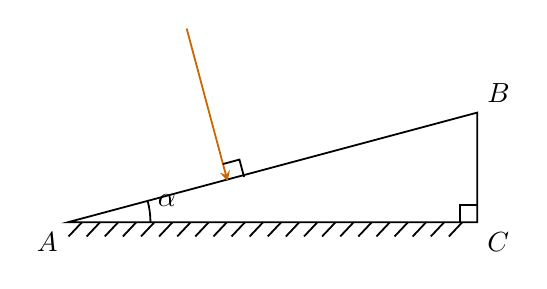
\begin{tikzpicture}[>=stealth,line width=.65pt]\draw (0,0)--(5.2,0)--(5.2,1.393)--cycle;\draw (1.05,0)arc(0:15:1.05)node[right]{$\alpha$};\foreach \x in {.18,.41,...,5.2}{\draw(\x,0)--++(-.17,-.18);}\draw (4.98,0)--(4.98,.22)--(5.2,.22);\draw[->,orange!80!black] (1.51,2.46)--(2.03,.52);\draw (1.971,.74)--(2.18,.796)--(2.239,.576);\node[below left]at(0,0){$A$};\node[above right]at(5.2,1.393){$B$};\node[below right]at(5.2,0){$C$};\end{tikzpicture}\end{center}

Нижняя грань AC прозрачного клина посеребрена и представляет собой плоское зеркало. Угол при вершине клина $\alpha = 15\ensuremath{{}^{\circ}}.$ Луч света падает из воздуха на клин перпендикулярно грани AB, преломляется и выходит в воздух через ту же грань AB, но уже под углом преломления $\beta = 60\ensuremath{{}^{\circ}}.$ Определите показатель преломления клина. Сделайте рисунок, поясняющий ход луча в клине.
}{
\smallskip\noindent\textbf{Решение}\par
\begin{center}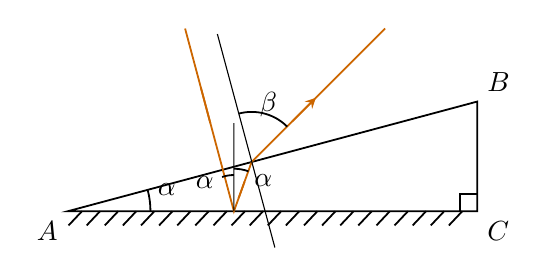
\begin{tikzpicture}[>=stealth,line width=.65pt]\draw (0,0)--(5.2,0)--(5.2,1.393)--cycle;\draw (1.05,0)arc(0:15:1.05)node[right]{$\alpha$};\foreach \x in {.18,.41,...,5.2}{\draw(\x,0)--++(-.17,-.18);}\draw (4.98,0)--(4.98,.22)--(5.2,.22);\draw[orange!80!black] (1.49,2.32)--(2.11,0)--(2.335,.626)--(4.03,2.32);\draw[->,orange!80!black](1.69,1.57)--(1.81,1.12) (2.17,.168)--(2.245,.375) (2.85,1.14)--(3.15,1.44);\draw[thin](2.11,0)--(2.11,1.12) (1.9,2.25)--(2.63,-.46);\draw (2.11,.46)arc(90:109:.46) (2.11,.54)arc(90:70:.54);\node[left]at(1.98,.37){$\alpha$};\node[right]at(2.24,.39){$\alpha$};\draw (2.17,1.24)arc(105:45:.638)node[above left]{$\beta$};\node[below left]at(0,0){$A$};\node[above right]at(5.2,1.393){$B$};\node[below right]at(5.2,0){$C$};\end{tikzpicture}\end{center}

$1$.  Луч, падающий на грань АВ, не преломляется, так как угол падения равен $0$\ensuremath{{}^{\circ}}. При падении на зеркальную грань $AC$ он падает под углом, который из геометрических соображений равен углу $\alpha .$ По закону отражения света угол отражения будет также равен $\alpha .$ 
$2$.  Данный луч падает на грань АВ под углом $\alpha _1=2 \alpha .$ По закону преломления света $\frac{\sin \alpha _1}{\sin \beta} = \frac{1}{n} ,$ откуда показатель преломления материала клина 

\[n= \frac{\sin \beta}{\sin 2 \alpha} = \frac{\sin 60 ^\circ}{\sin ( 2 \cdot 15 ^\circ )} = \sqrt{3} \approx 1{,}73.\]

Ответ: $1{,}73$.
}

\end{document}
